
\chapter{Complementary Searches and Outlook}
\label{ch:Conclusion}
%Deep thoughts go here.
\section{Comparison with Complementary Searches}
\section{Future Directions}
HL-LHC and Beyond
Future prospectives at Linear Colliders?
\section{Conclusion}


%
%%%%%%%%%%%%%%%%%%%%%%%%%%%%%%%%%%%%%%%%%%%%%%%%
%%%%%%%%%%%%%                                                                                                   %%%%%%%% 
%%%%%%%%%%%%%                           BEN                                                                  %%%%%%%% 
%%%%%%%%%%%%%                                                                                                   %%%%%%%% 
%%%%%%%%%%%%%%%%%%%%%%%%%%%%%%%%%%%%%%%%%%%%%%%%
%
%This chapter contains co-authored material from Refs.~\cite{DijetISR_Resolved}\cite{DijetTLA}\cite{DijetISR}, written as part of the ATLAS Collaboration.
%\newline
%
%The high-mass dijet search is just one piece of the strategy to search for new resonances which decay to dijet final states.  ATLAS has several other recently-published searches for dijet events which probe the lower-mass regime, an area inaccessible in this search due to the kinematic limitation of the trigger used.  These searches combine to set limits on new resonances down to 100\,GeV.
%
%\section{Trigger-Level Analysis}
%The ATLAS trigger-level analysis uses the technique of data scouting to collect dijet events with lower \pt jets than can be normally saved.  Data scouting gets around the trigger rate limitation by only saving a small portion of the event, usually just the jets used in the high-level trigger and some global event quantities, rather than the full set of physics objects and detector information.  This creates a much smaller event size and allows for a much larger dataset to be collected than is normally possible, at the expense of not having the standard fully-calibrated jets to use in the analysis.  A series of calibrations is used to bring these trigger-level jets close to the quality of offline jets.  The very high statistics provided by this dataset has also revealed limitations in parts of the standard jet calibration sequence, such as the need for a smoother jet energy scale in-situ calibration to prevent the calibration from introducing bumps into the invariant mass spectrum.  The comparison between the the standard JES and the new smoothed fit it shown in Figure~\ref{fig:JES_TLA}.  This new, smoother in-situ calibration will be needed in the high-mass dijet analysis for future results as the amount of data increases even further, increasing the sensitivity of the search to such tiny fluctuations.
%
%\begin{figure}[ht!]
%	\centering
%	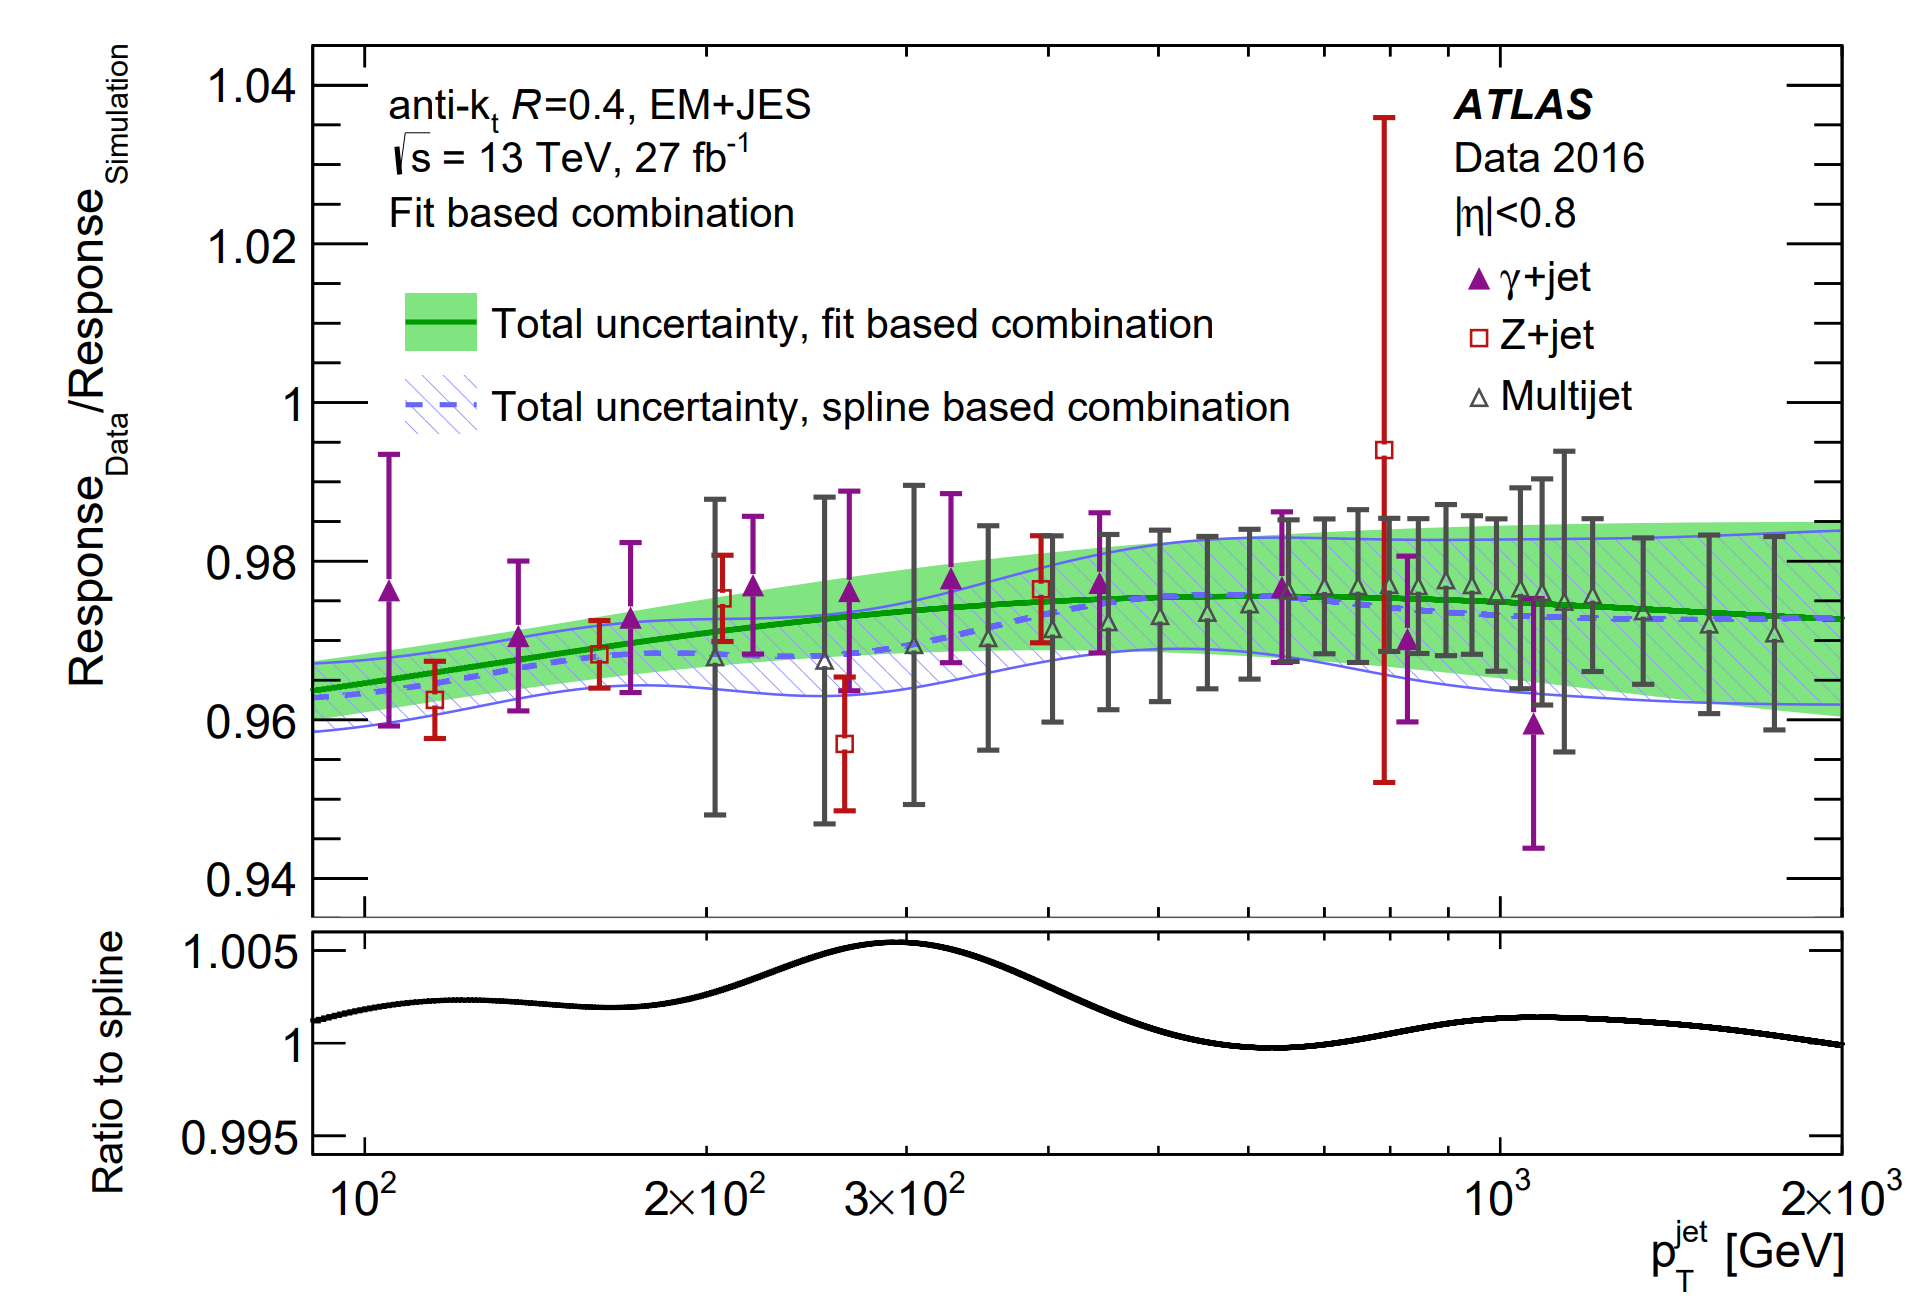
\includegraphics[width=0.7\columnwidth]{figures/Conclusion/JES_TLA.png}
%	\caption{In-situ calibration in the range of 85\,GeV $<$ jet \pt $<$ 2\,TeV for both the traditional spline method (dashed line) and new fitted (solid line) combination methods.  Data points from the three input measurements are overlaid.  The lower panel shows the ratio of the two calibration curves.}
%	\label{fig:JES_TLA}
%\end{figure}
%
%The trigger-level analysis uses a similar series of cuts as the standard dijet analysis, analyzing events with a leading jet with $\pt > 220$\,GeV and a second jet with $\pt > 85$\,GeV, with $|y^*|<$0.6, and in the invariant mass range 700\,GeV $< \mjj <$ 1800\,GeV.  The analysis also has a second search region which uses data taken in early 2016 with a lower-threshold trigger.  This region lowers the leading jet cut to $\pt > 185$\,GeV, with $|y^*| <$ 0.3 and probes the region $\mjj > 450$\,GeV.  The results of the search are shown in Figure~\ref{fig:TLA_Search}, and limits obtained for the $Z'$ dark matter mediator in the two search regions are shown in Figure~\ref{fig:TLA_Limits}, along with a comparison to the result obtained from the high-mass dijet search.\cite{DijetTLA}
%
%\begin{figure}[ht!]
%	\centering
%	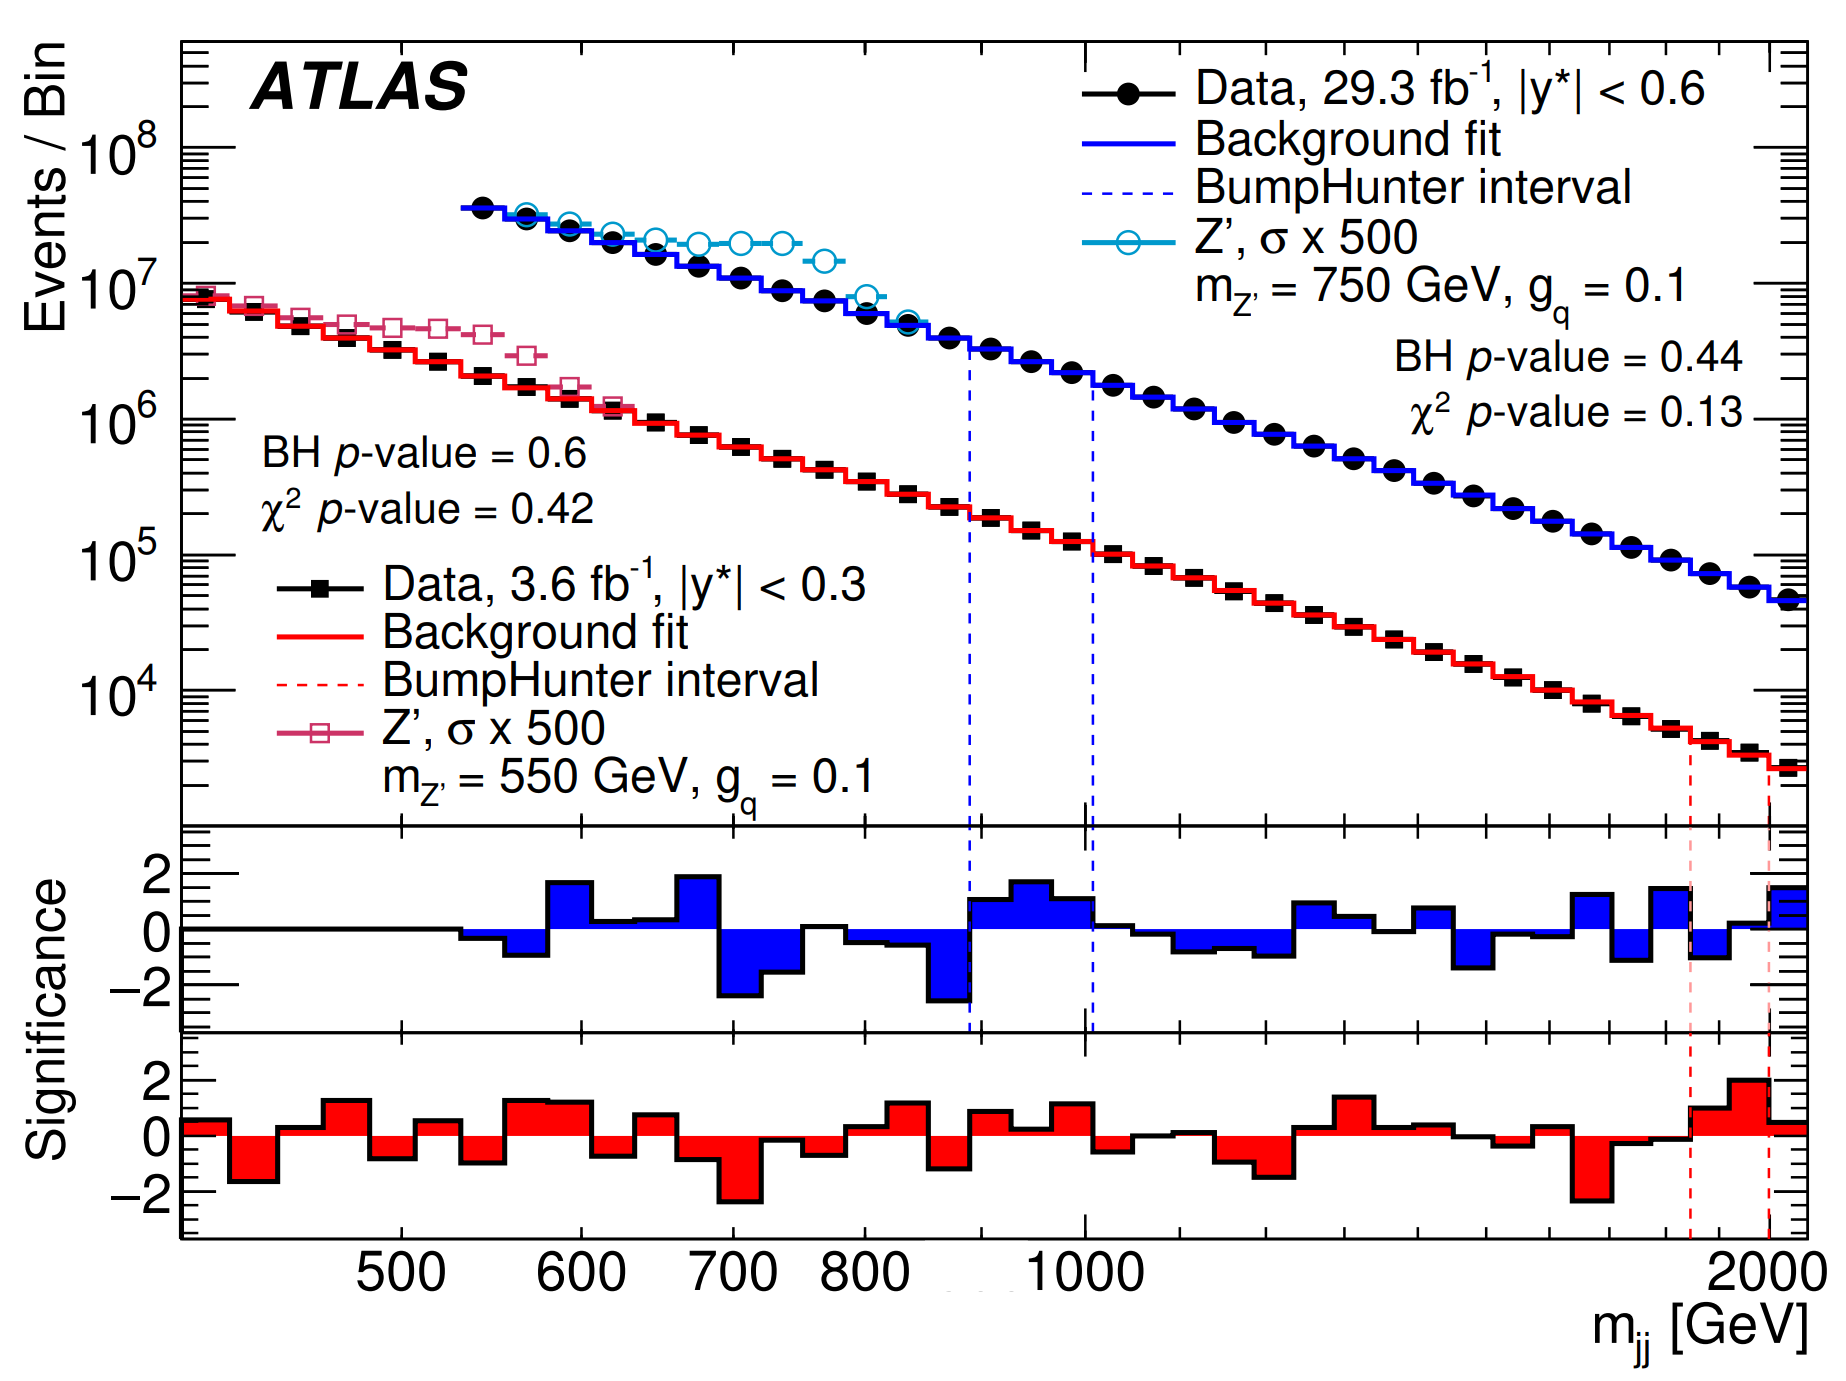
\includegraphics[width=0.7\columnwidth]{figures/Conclusion/TLA_Search.png}
%	\caption{Reconstructed dijet mass distribution for events in the $|y^*|<0.3$ (red) and $|y^*|<0.6$ (blue) signal regions.  The solid lines depict the background estimate obtained by a sliding window fit.  The lower panel shows the bin-by-bin significances of the differences between the data and the background estimate, and the most discrepant region in both signal regions is indicated by the colored vertical lines.}
%	\label{fig:TLA_Search}
%\end{figure}
%
%\begin{figure}[ht!]
%	\centering
%	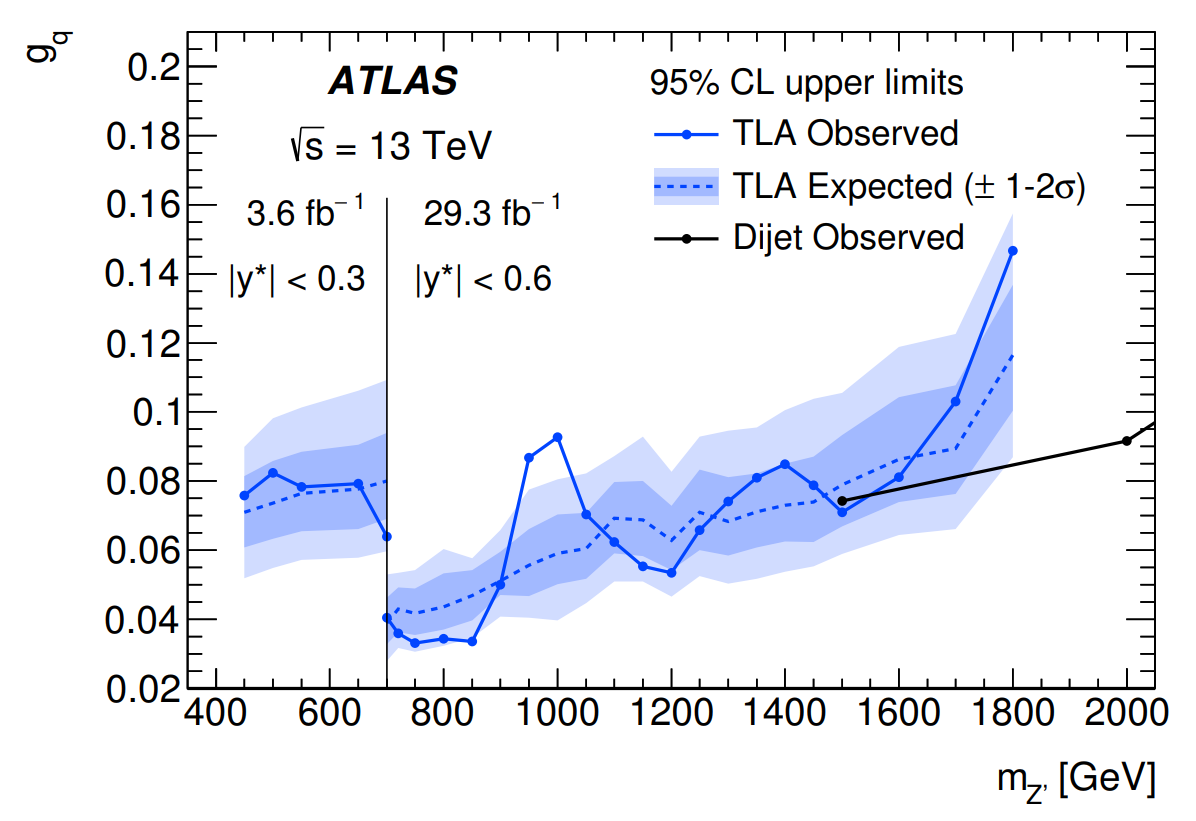
\includegraphics[width=0.7\columnwidth]{figures/Conclusion/TLA_Limits.png}
%	\caption{The 95\% credibility-level observed and expected upper limits on $g_q$ as a function of $m_{Z'}$.  The lower-mass portion of the limits from the high-mass dijet result is also shown.  Couplings above the solid lines are excluded.}
%	\label{fig:TLA_Limits}
%\end{figure}
%
%\section{Dijet + Initial State Radiation Searches}
%
%To probe an even lower energy regime, ATLAS has performed two other searches which look for resonances in association with initial state radiation.  This circumvents the trigger limitation by triggering on a high-\pt photon or jet rather than on the much softer jets from the new resonance.  The first is the resolved dijet+ISR search which looks for two R=0.4 jets in association with a high-\pt jet or photon.\cite{DijetISR_Resolved}  The results of that search are shown in Figures~\ref{fig:ISR_Resolved} and~\ref{fig:ISR_Resolved_Limits}. The other is the boosted search which looks for one large radius (R=1.0) jet rather than for two distinct R=0.4 jets.\cite{DijetISR}  Background processes are suppressed by cutting on jet substructure variables which measure the likelihood that the energy deposition within the large jet is from two sub-jets rather than from the single jet expected from QCD background.  The results of the search are shown in Figure~\ref{fig:ISRSearch}.  This search is used to set limits on the same $Z'$ dark matter mediator model between 100 and 220\,GeV, and the results are shown in Figure~\ref{fig:ISRLimits}.
%
%\begin{figure}[ht!]
%	\centering
%	\subfloat[]{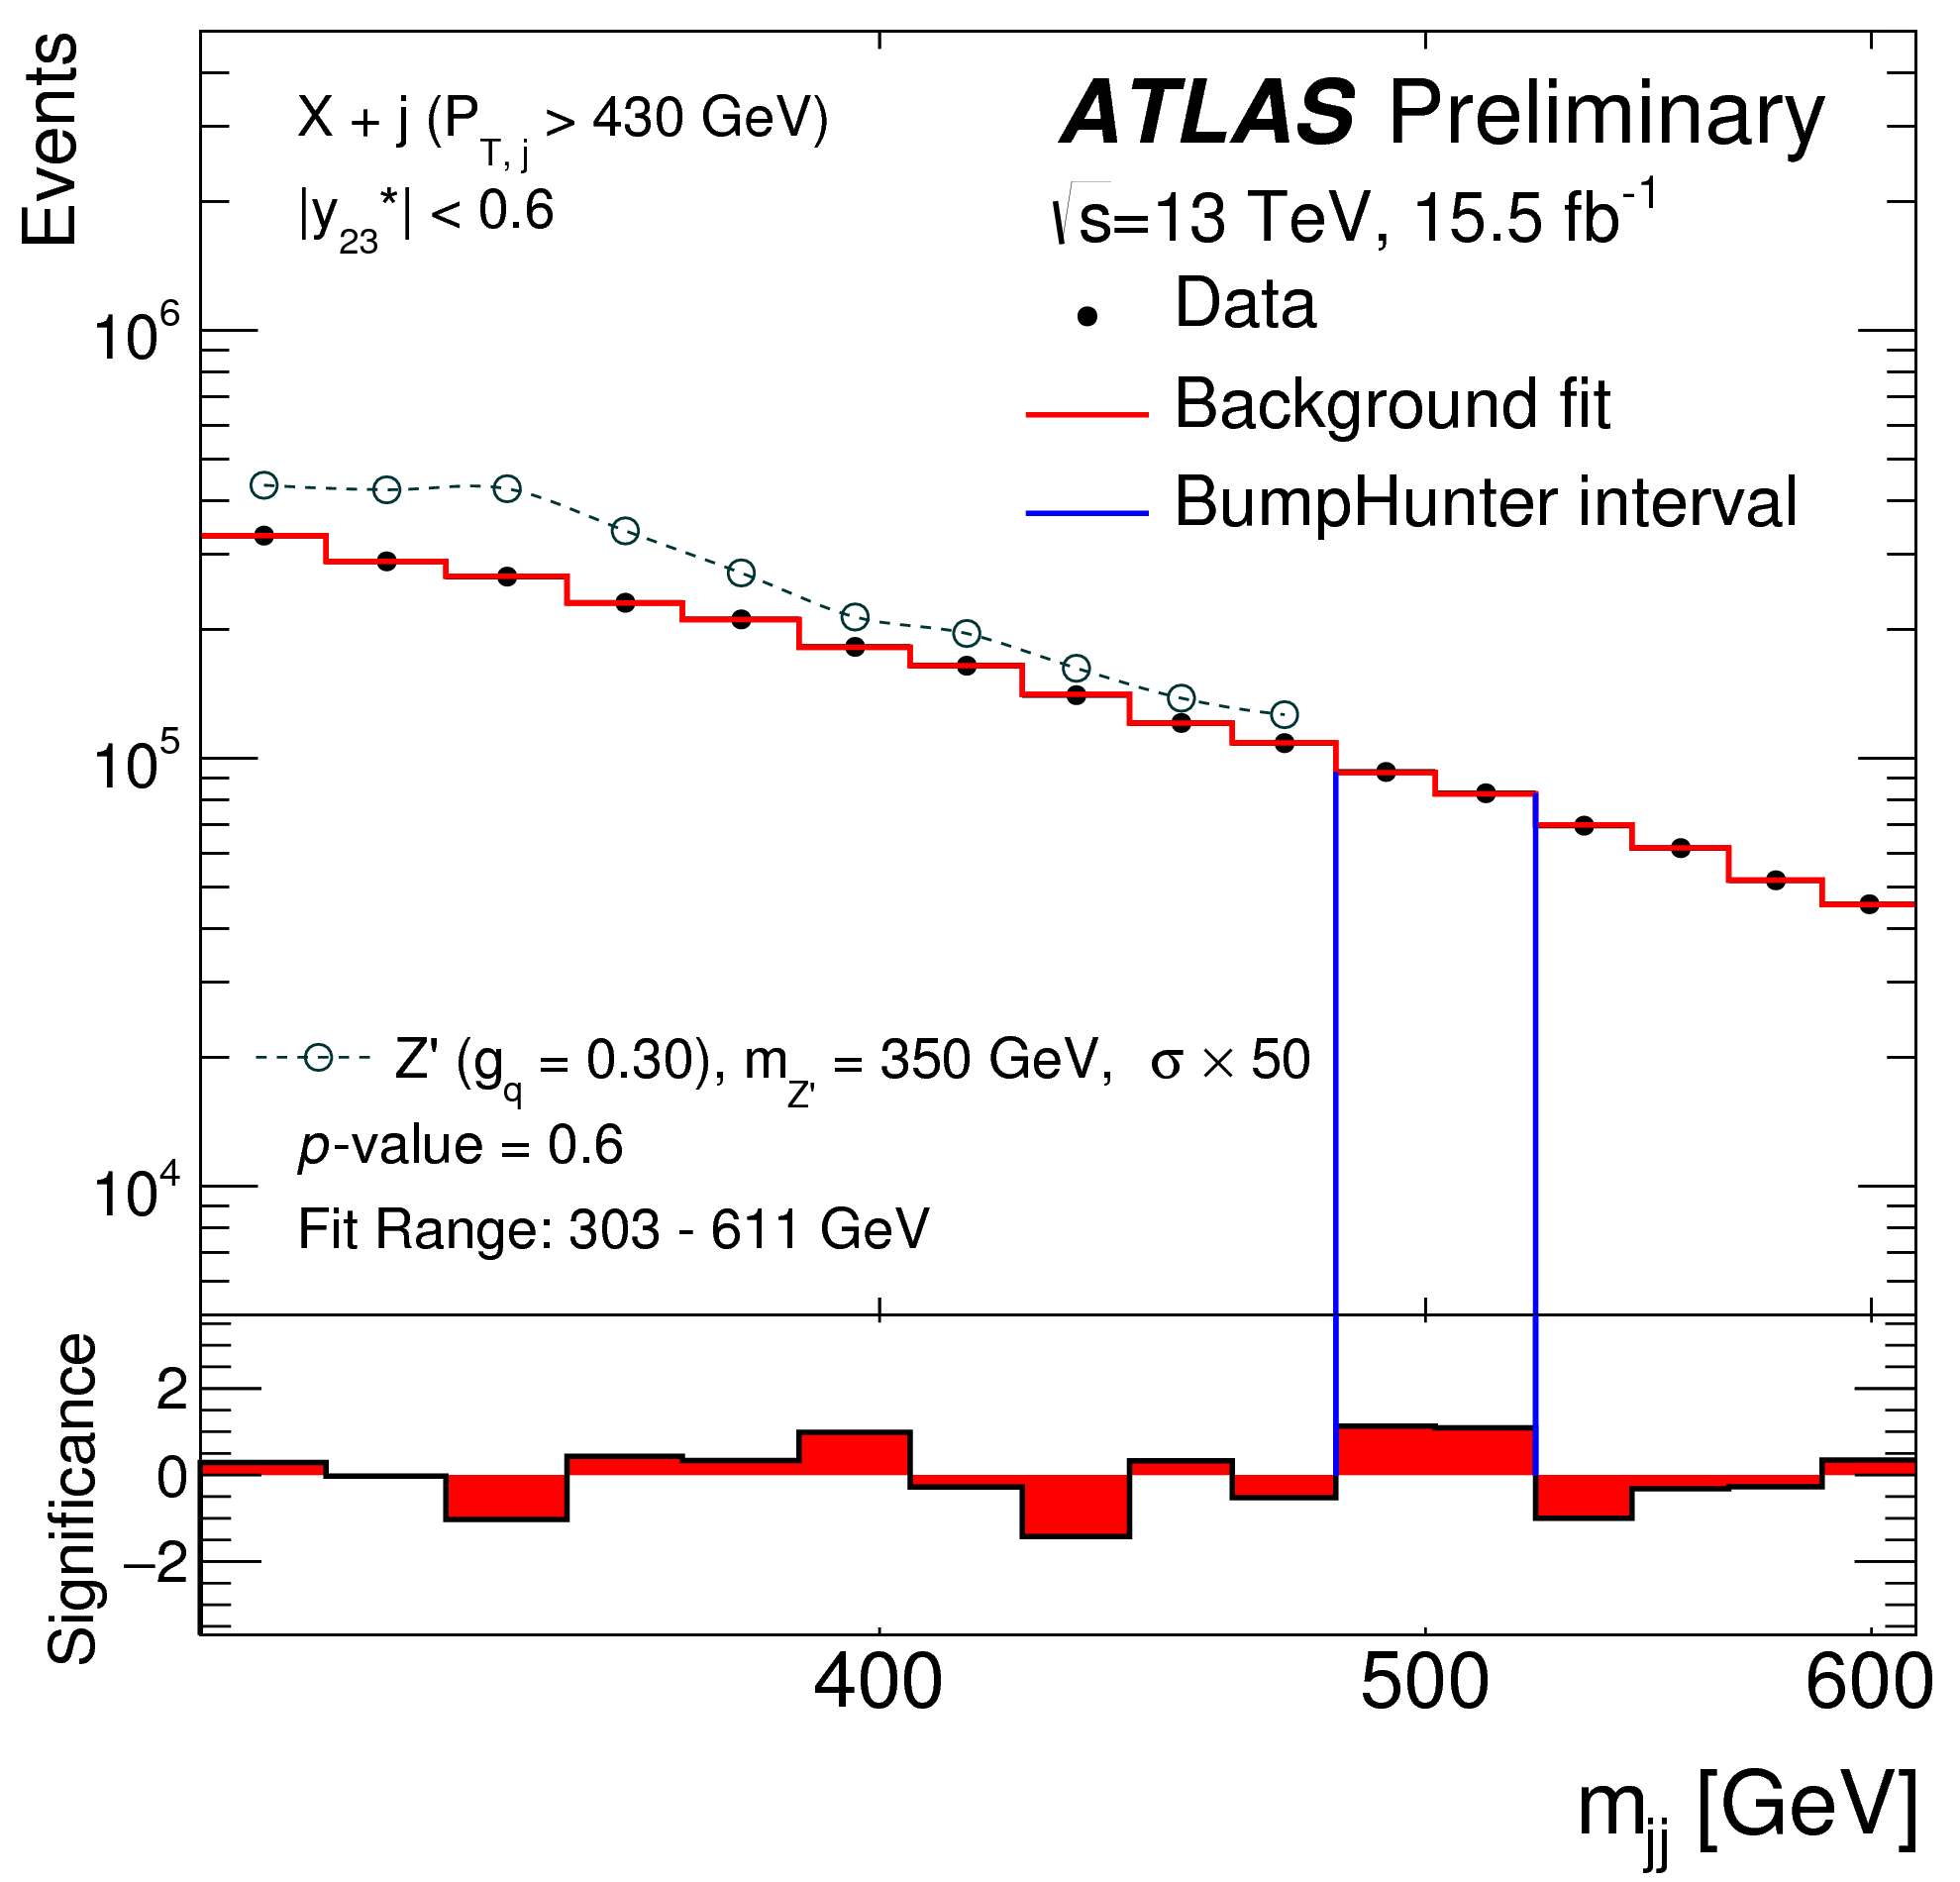
\includegraphics[width=0.45\columnwidth]{figures/Conclusion/ResolvedJetSearch.png}}
%	\hspace{0.1\textwidth}%
%	\subfloat[]{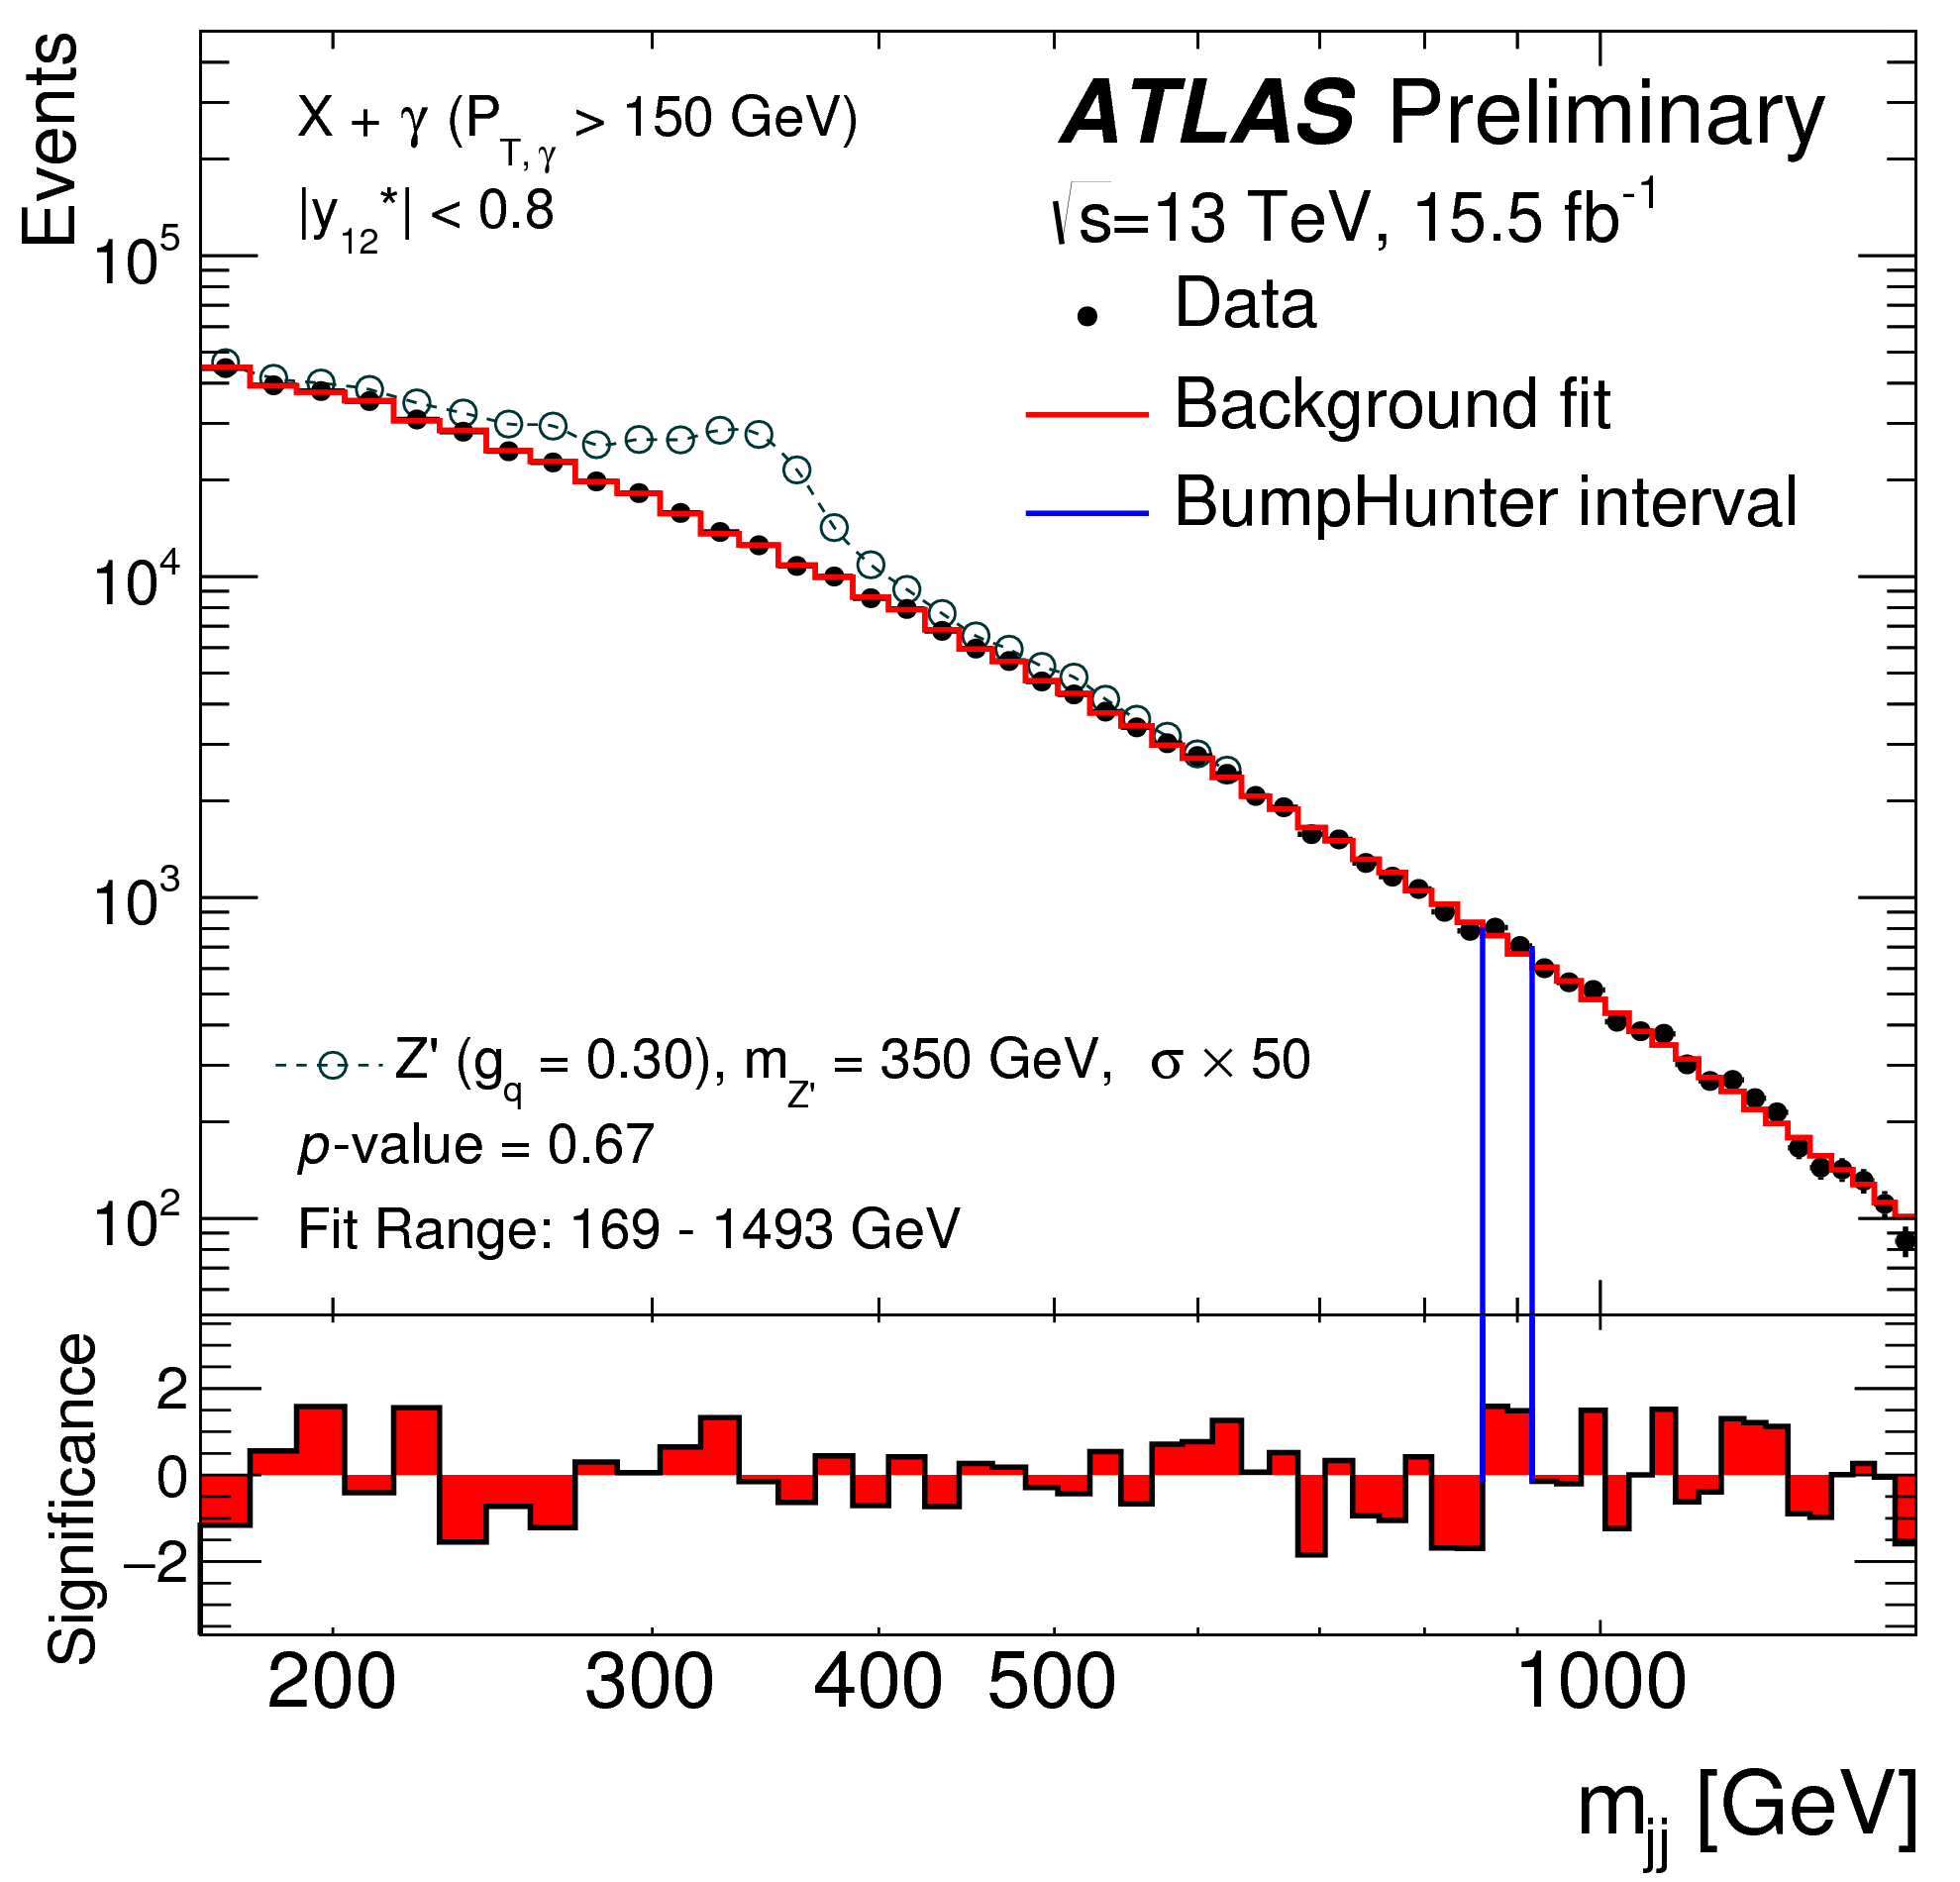
\includegraphics[width=0.45\columnwidth]{figures/Conclusion/ResolvedPhotonSearch.png}}
%	\caption{Reconstructed dijet mass distribution for events containing two jets with $\pt > 25$\,GeV and either a jet with $\pt > 430$\,GeV (left) or a photon with $\pt > 150$\,GeV (right).  The vertical lines indicate the most discrepant region as identified by the BumpHunter algorithm, and the bottom panel shows the bin-by-bin significances of the data with respect to the background fit.}
%	\label{fig:ISR_Resolved}
%\end{figure}
%
%\begin{figure}[ht!]
%	\centering
%	\subfloat[]{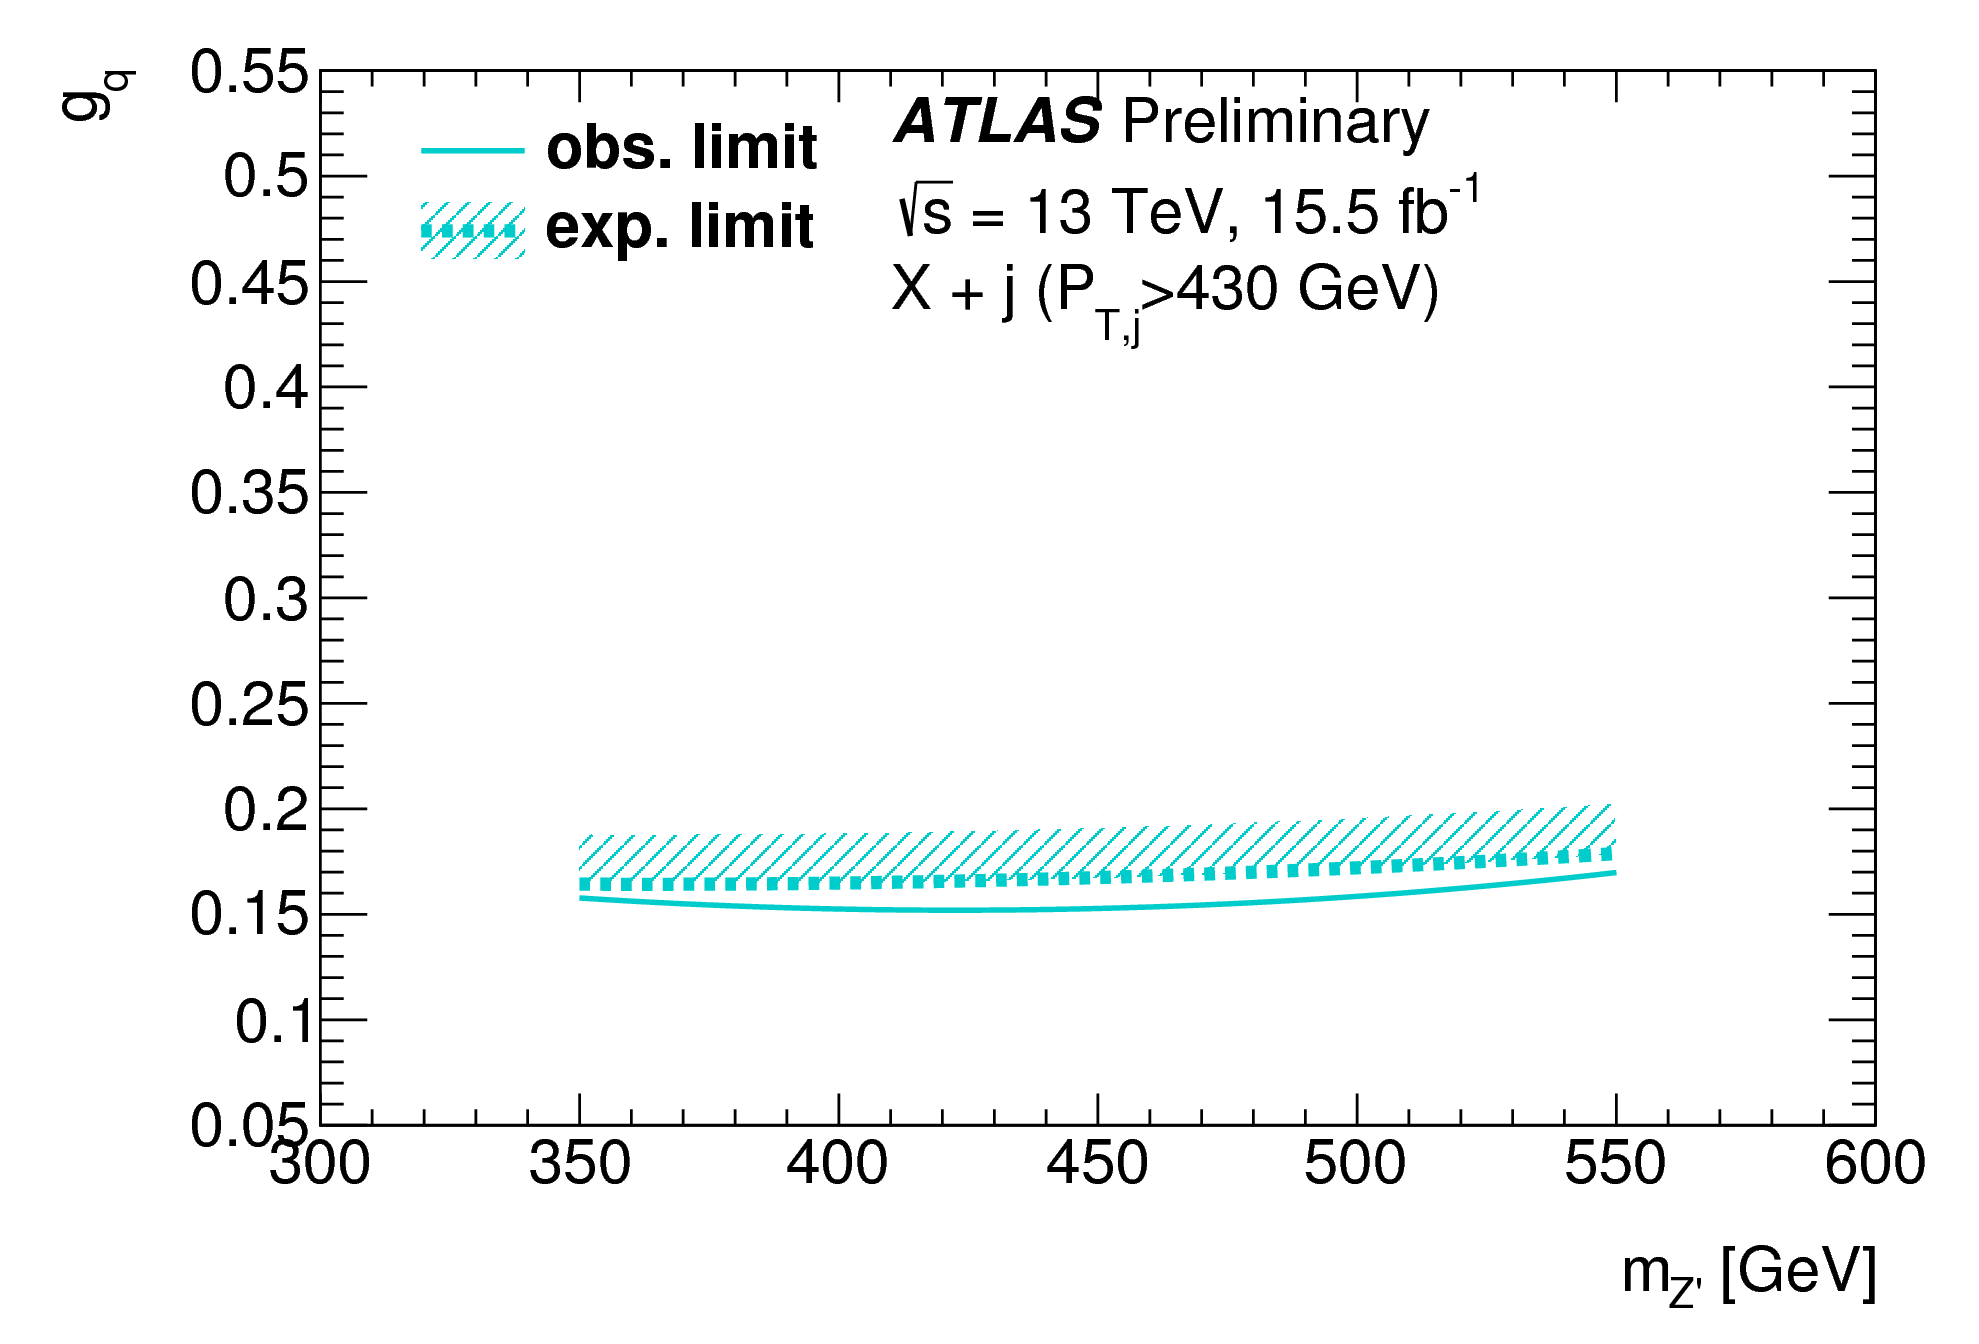
\includegraphics[width=0.45\columnwidth]{figures/Conclusion/ResolvedJet.png}}
%	\hspace{0.1\textwidth}%
%	\subfloat[]{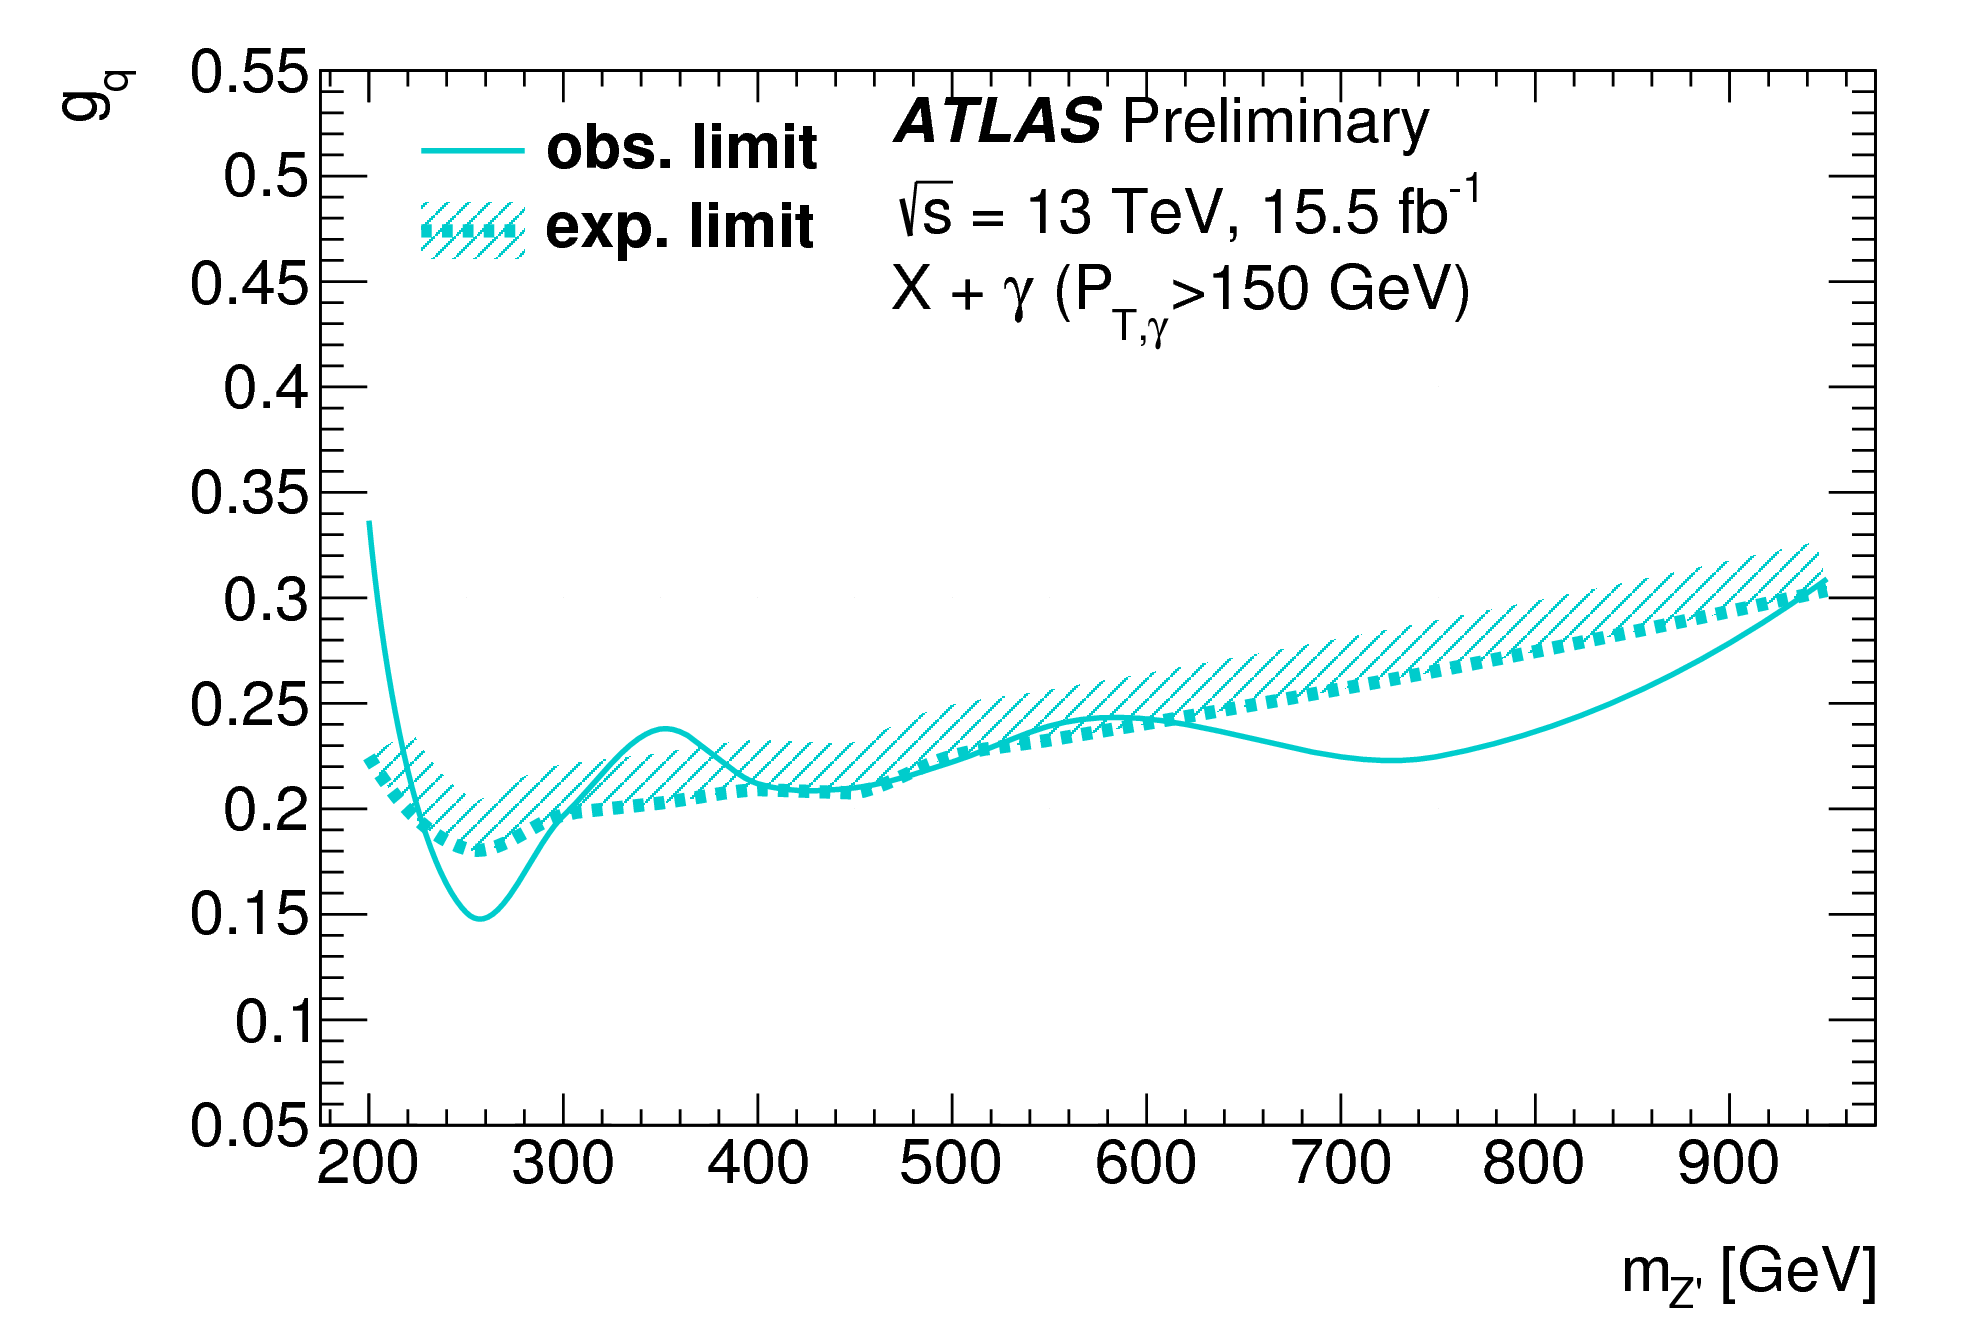
\includegraphics[width=0.45\columnwidth]{figures/Conclusion/ResolvedPhoton.png}}
%	\caption{The 95\% CL upper limits obtained from the X+jet (left) and X+photon (right) searches on coupling $g_q$ as a function of the resonance mass $m_{Z'}$ for the leptophobic $Z'$ dark matter mediator model.}
%	\label{fig:ISR_Resolved_Limits}
%\end{figure}
%
%\begin{figure}[ht!]
%	\centering
%	\subfloat[]{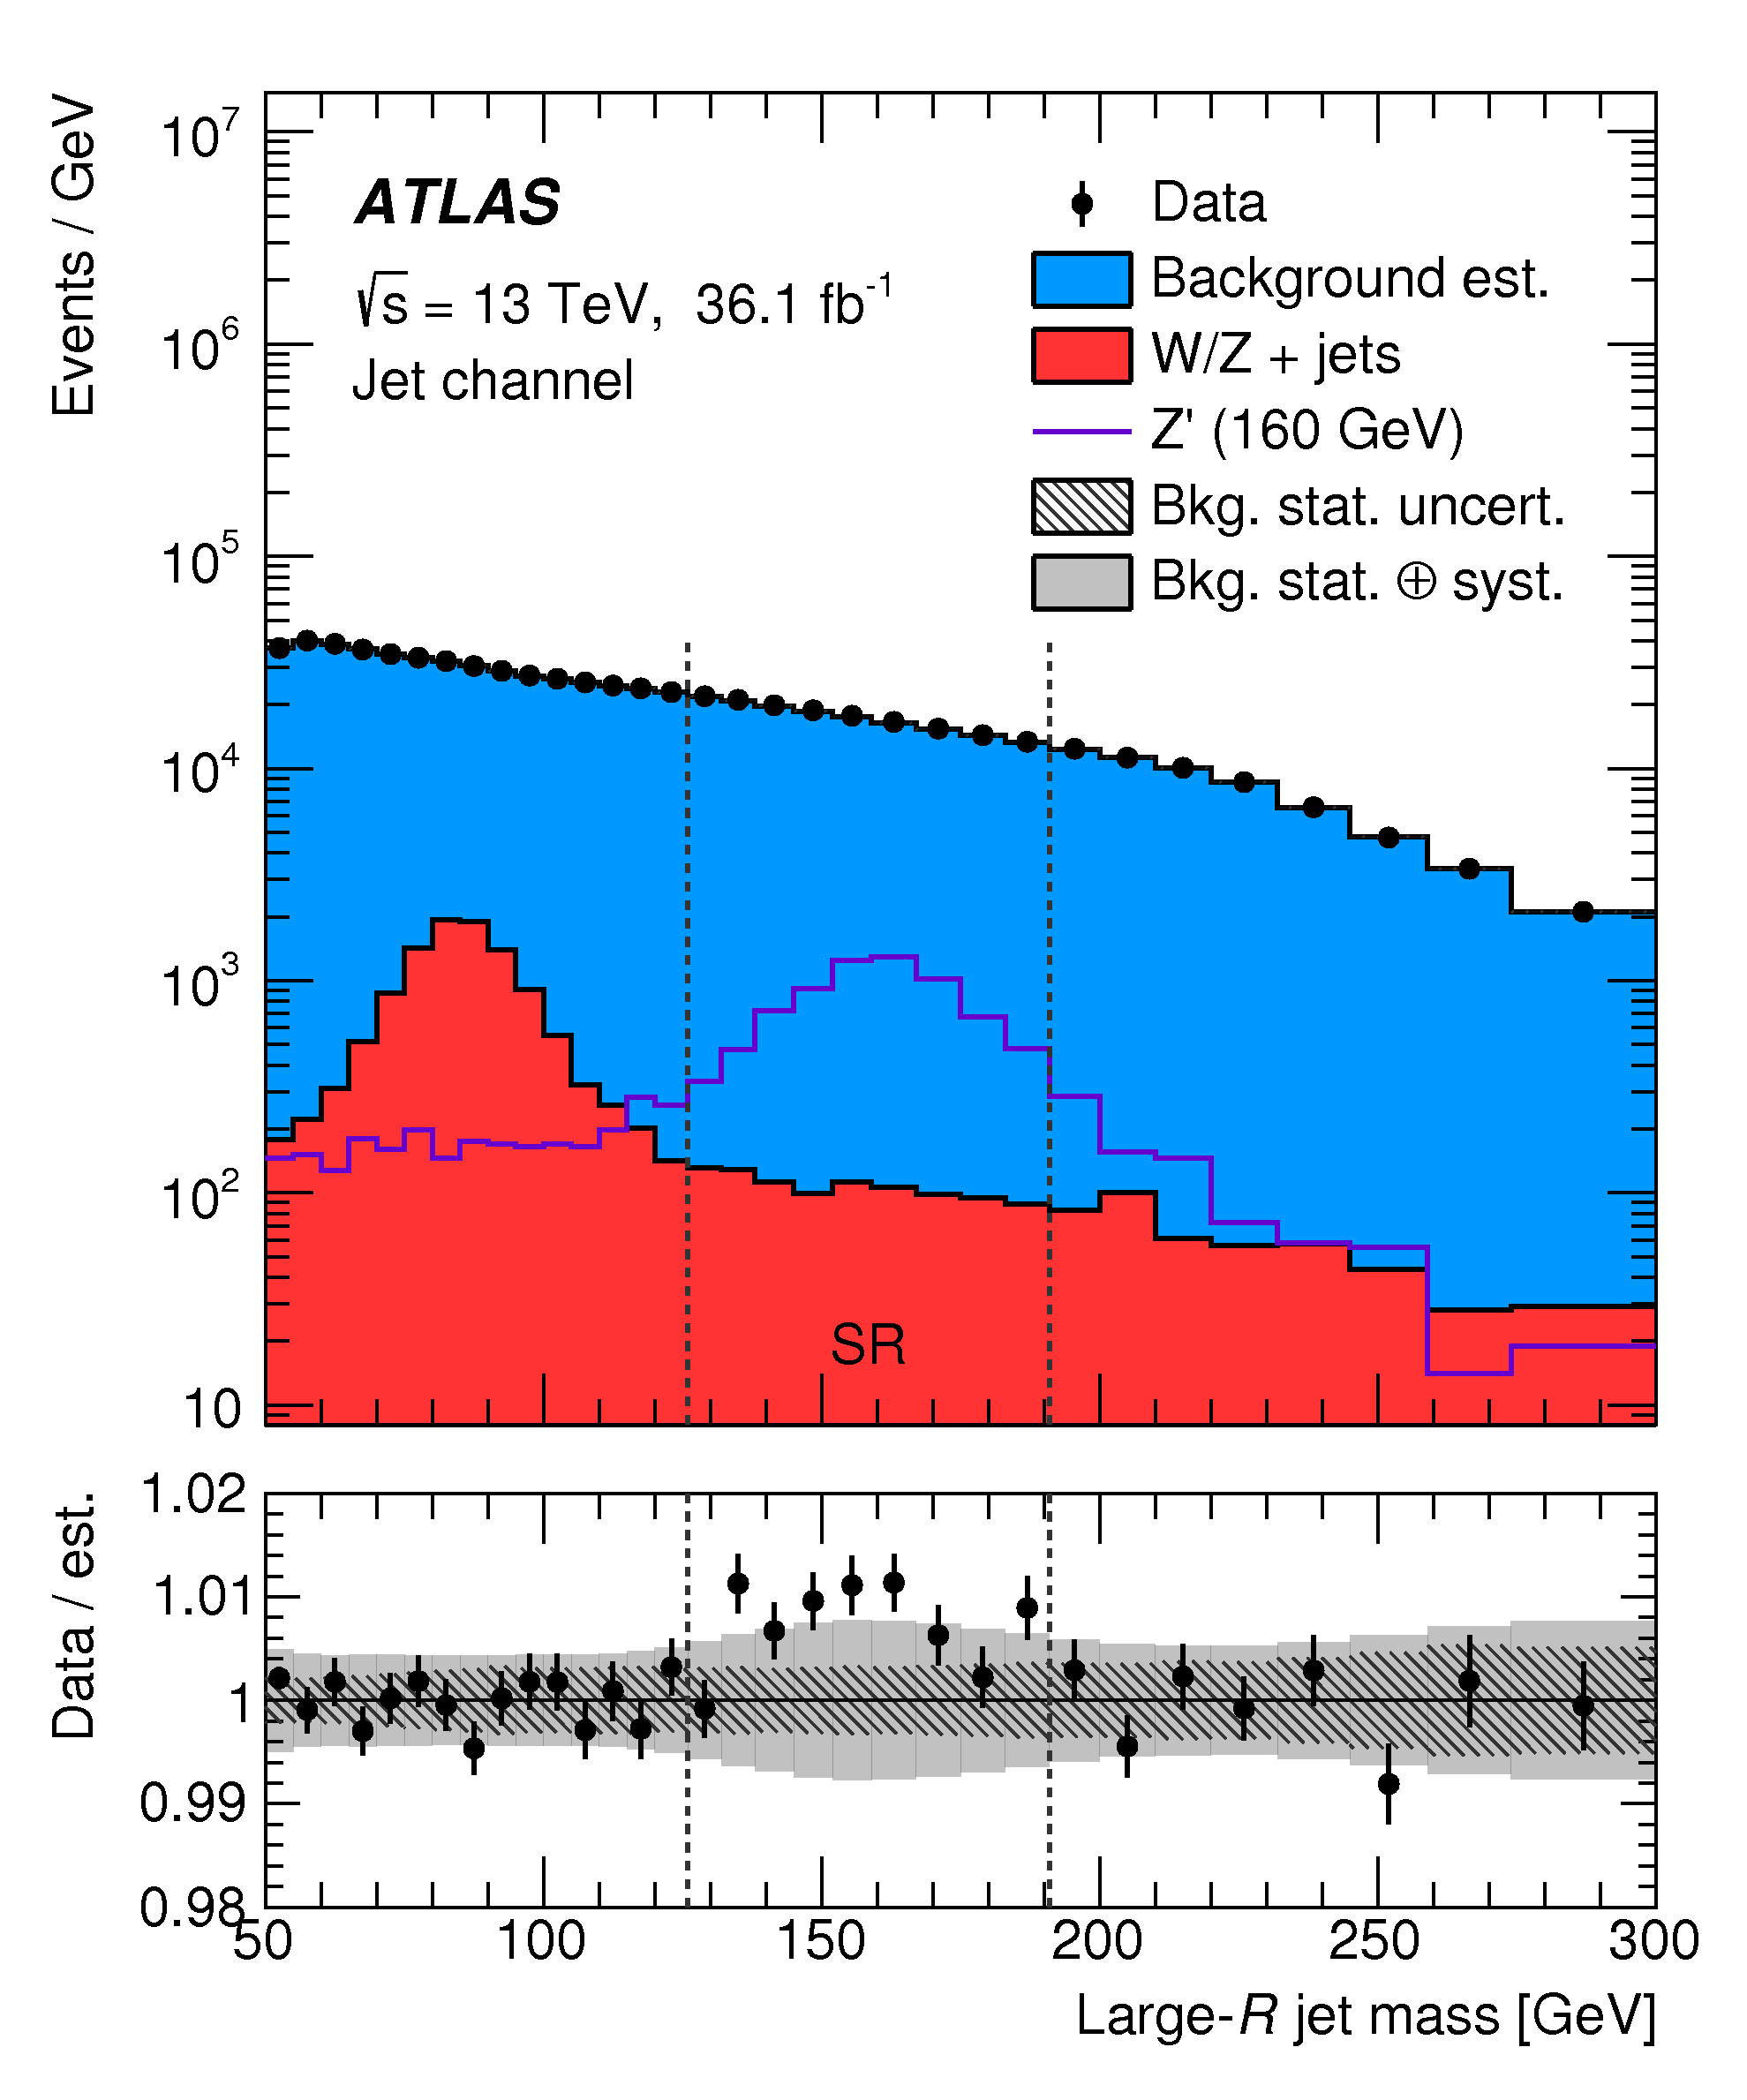
\includegraphics[width=0.45\columnwidth]{figures/Conclusion/ISRJet.png}\label{subfig:ISRJet}}
%	\hspace{0.1\textwidth}%
%	\subfloat[]{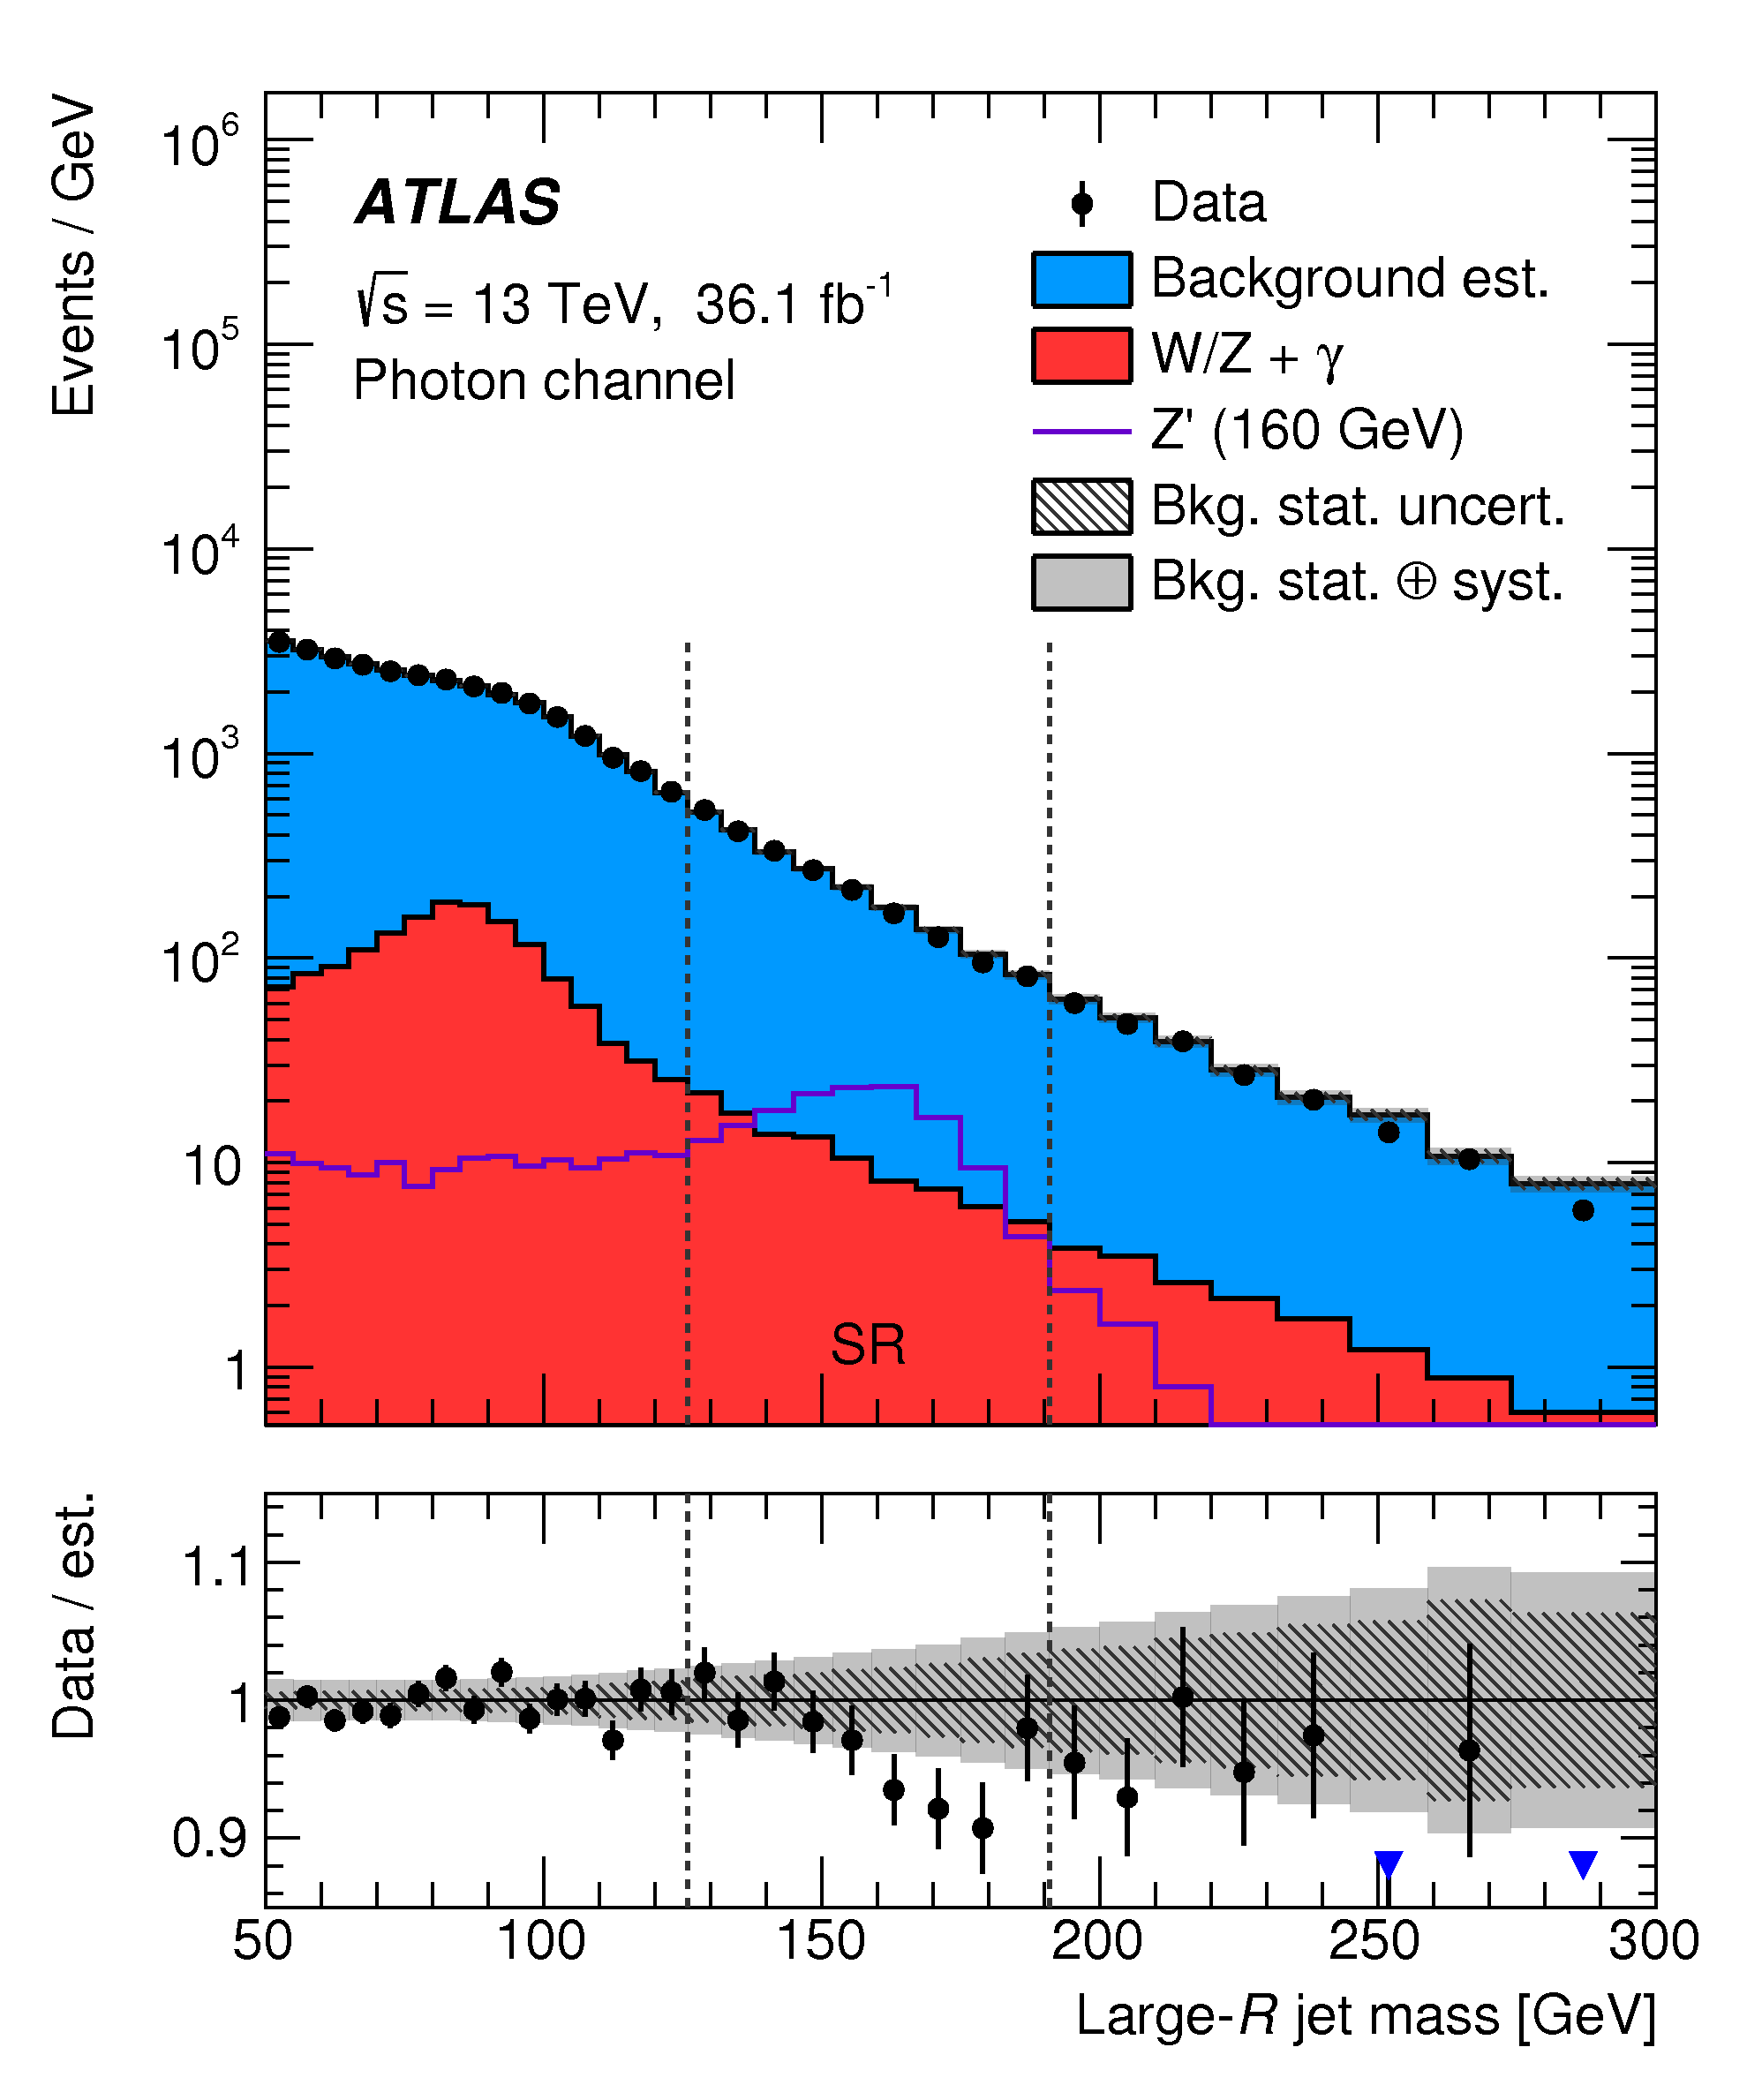
\includegraphics[width=0.45\columnwidth]{figures/Conclusion/ISR_Photon.png}\label{subfig:ISRPhoton}}
%	\caption{Distribution of Large-R jet mass in the ISR jet (left) and ISR photon (right) channels.  The signal $Z'$ shown has a mass of 160\,GeV and coupling $g_q$=0.5.  The bottom panel shows the ratio of the data to the estimated background; the estimate varies for different signal masses.}
%	\label{fig:ISRSearch}
%\end{figure}
%
%\begin{figure}[ht!]
%	\centering
%	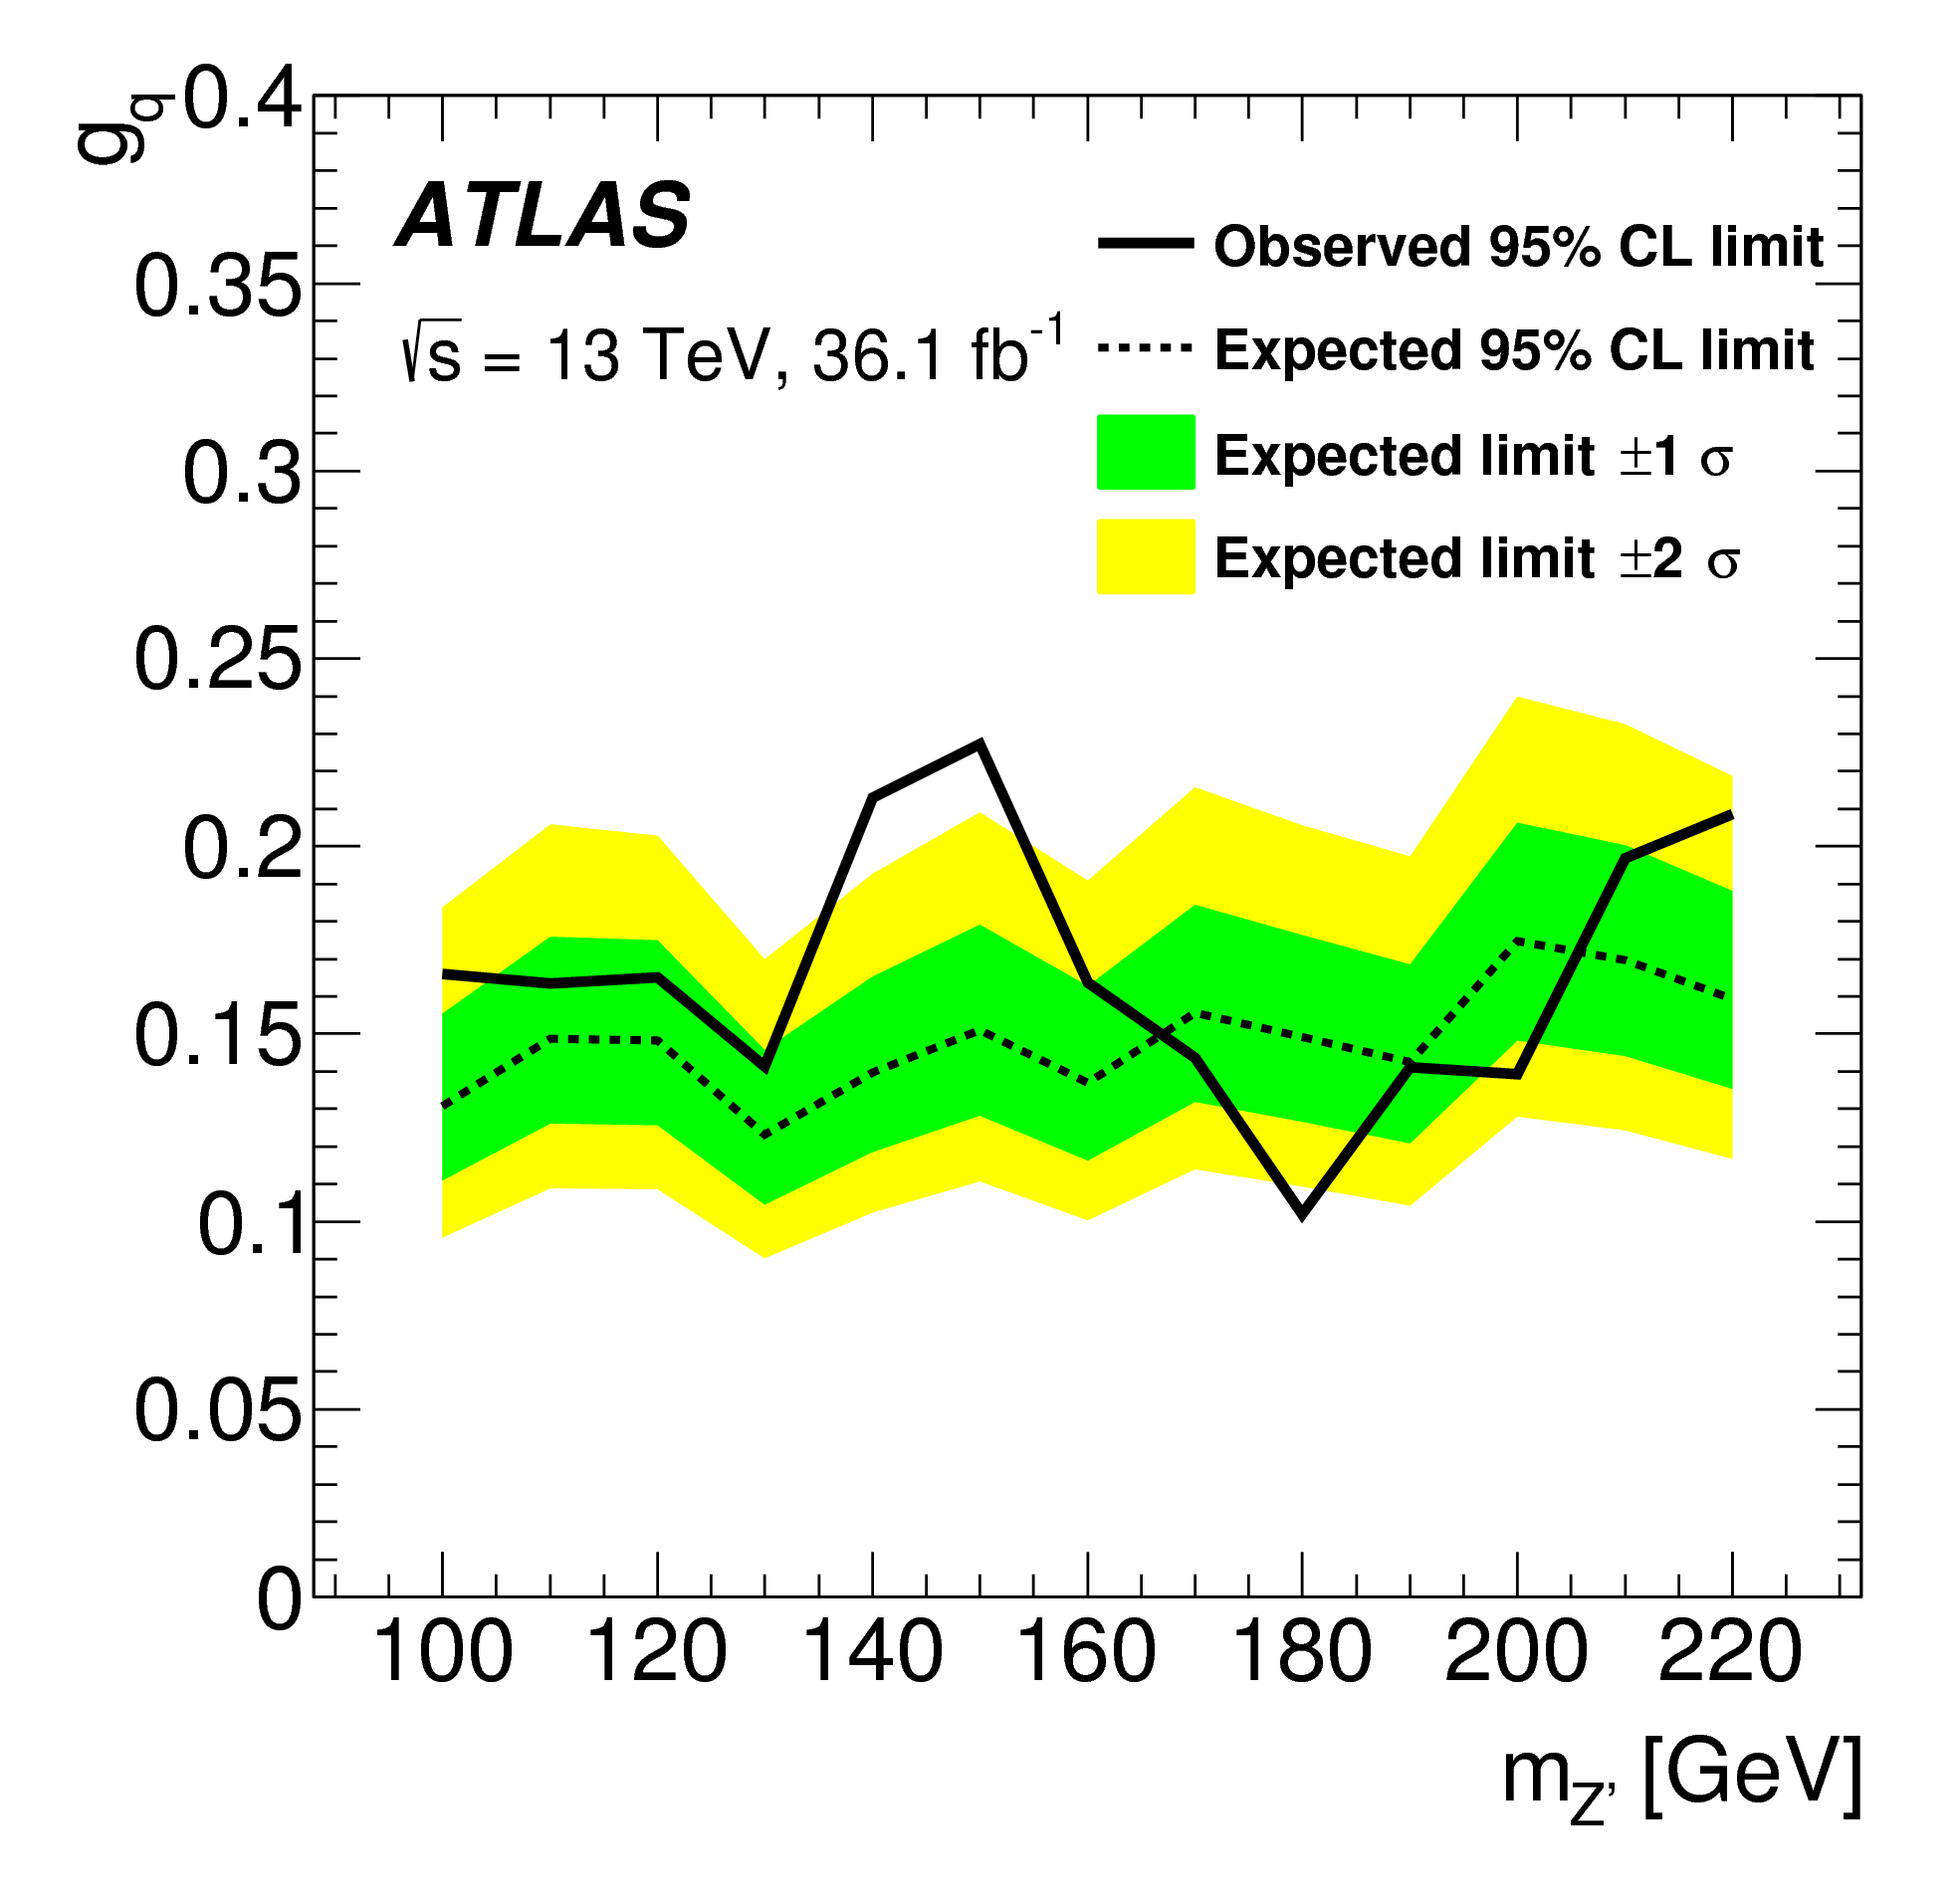
\includegraphics[width=0.6\columnwidth]{figures/Conclusion/ISR_Limits.png}
%	\caption{Observed and expected limits at 95\% CL on the coupling to quarks $g_q$ for the combined ISR jet and photon channels for the boosted search. }
%	\label{fig:ISRLimits}
%\end{figure}
%
%\section{Combined limits on Dark Matter Models}
%
%The limits set on the $Z'$ dark matter mediator model by the dijet analysis, combined with the results from the aforementioned complimentary analyses, provide strong constraints on the model across a wide range of mediator masses.  Figure~\ref{fig:DMExclusions} shows the state of the analyses as of July 2017 following the release of the high-mass dijet result, but does not include the latest results from the dijet+ISR and TLA searches.  This  plot shows the limits for the $Z'$ model with coupling $g_q$=0.25, shown in the plane of mediator ($Z'$) mass and the dark matter mass.  For this particular benchmark model, mediator masses between 200\,GeV and 2.6\,TeV have been excluded for all shown dark matter masses.  The various colors represent the regions excluded by the different results and help demonstrate the complementarity between the various ATLAS searches.  The very low mediator mass region is probed by a different class of searches which look for decays of the mediator to the dark matter particle in association with some kind of initial state radiation, such as the diagram in Figure~\ref{subfig:FeynmanMedToDM}.
%
%\begin{figure}[]
%	\centering
%	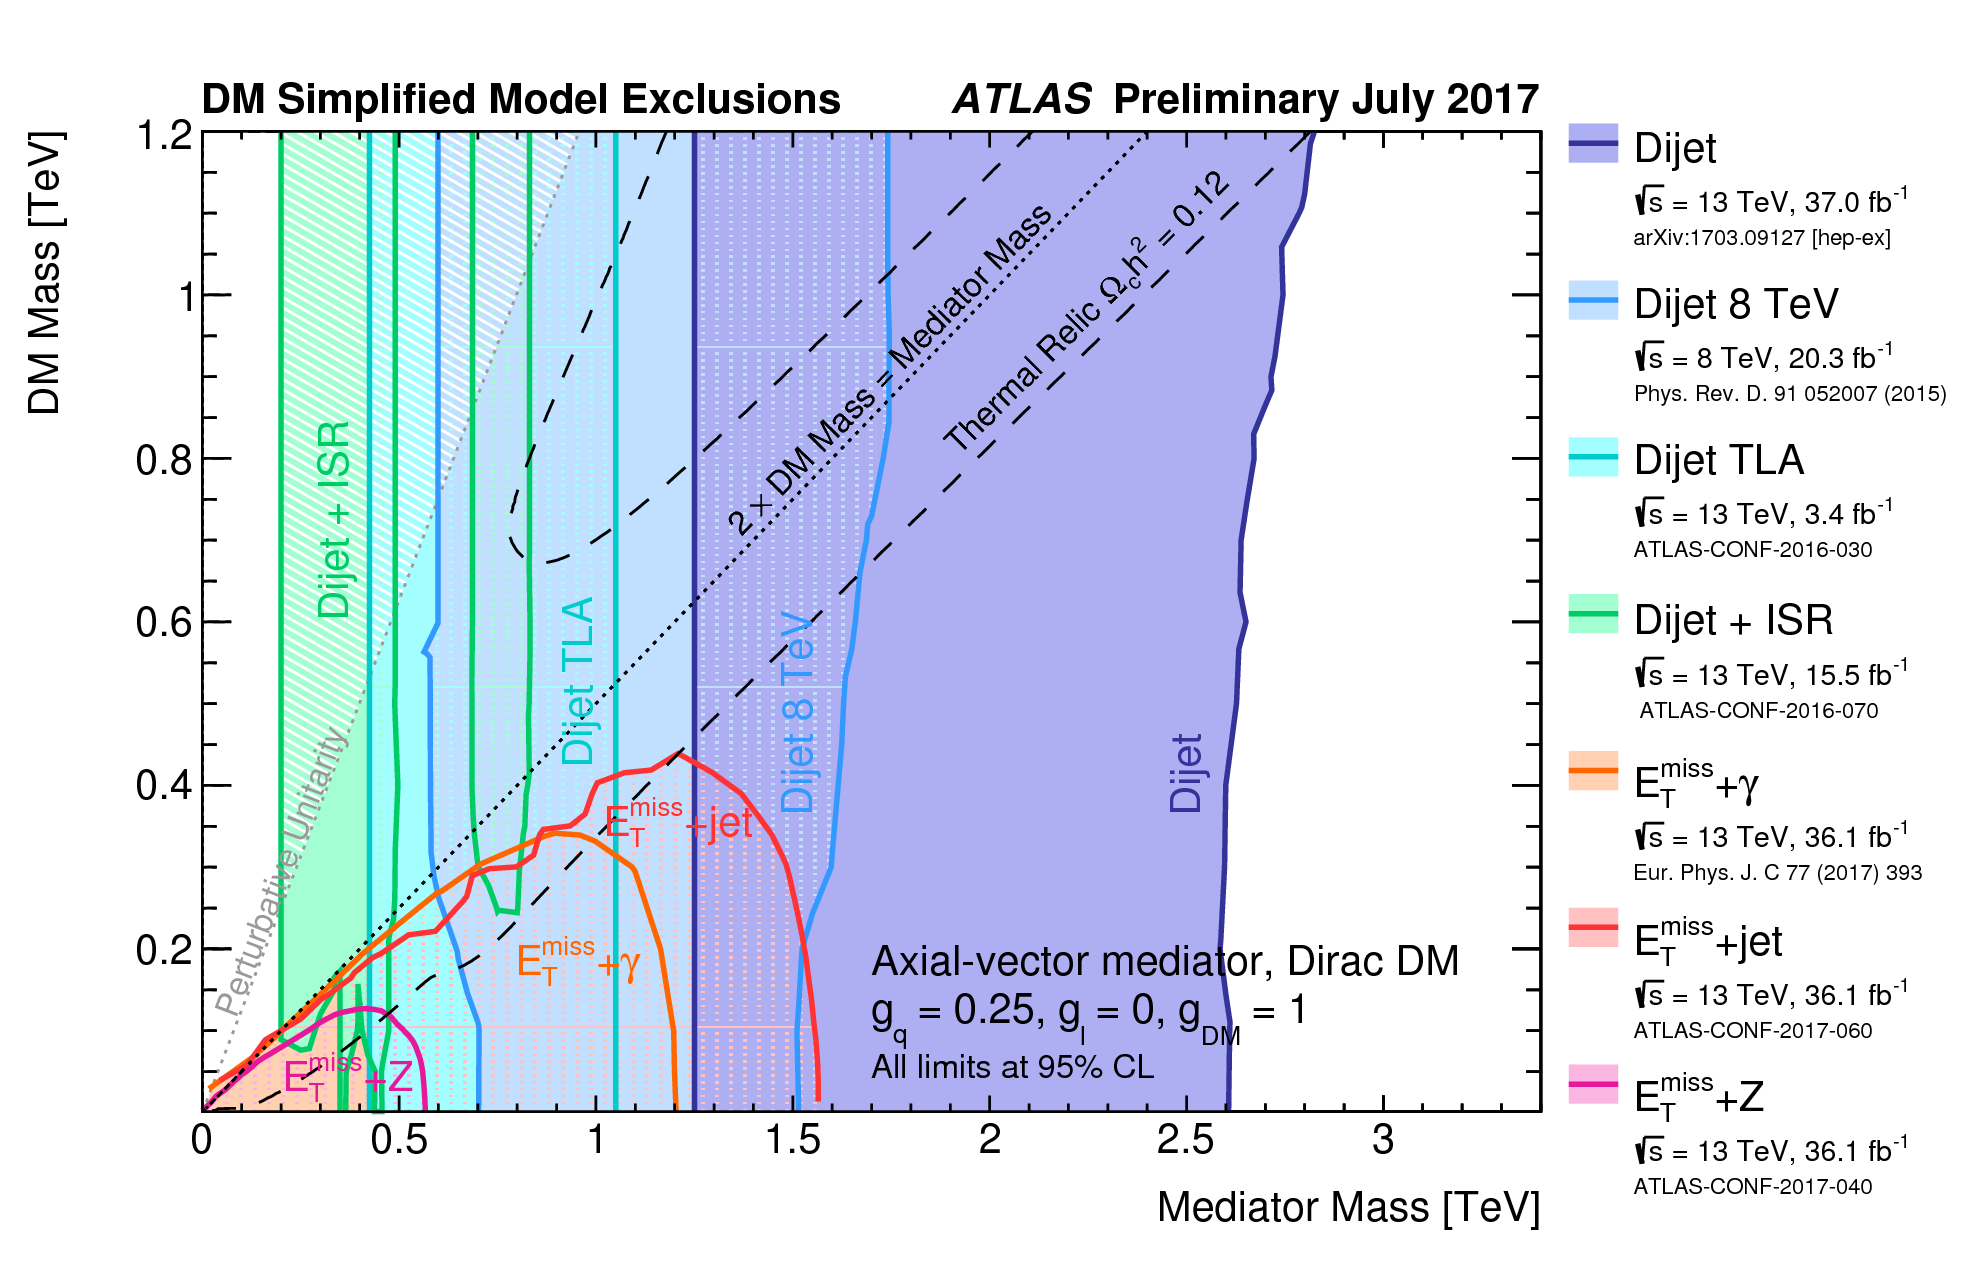
\includegraphics[width=\columnwidth]{figures/Conclusion/DMExclusions.png}
%	\caption{Regions in a dark matter mass-mediator mass plane excluded at 95\% CL by a selection of ATLAS dark matter searches, for one possible interaction between the Standard Model and dark matter, the leptophobic axial-vector mediator as described in \cite{DMWorkingGroup}. The exclusions are computed for a dark matter coupling $g_{DM}$ = 1.0, a quark coupling $g_q$ = 0.25 universal to all flavors. The lepton coupling $g_l$ in this model is set to zero. This choice for the couplings corresponds to the "A1" scenario in \cite{DMWorkingGroup}. The results use 13\,TeV data except for \cite{DijetResonance8TeV_ATLAS}. Dashed curves labeled "thermal relic" indicate combinations of dark matter and mediator mass that are consistent with a dark matter density of $\Omega_c = 0.12 h^2$ and a standard thermal history, as computed in MadDM (\cite{MadDM}, \cite{DMWorkingGroup}). Between the two curves, annihilation processes described by the simplified model deplete $\Omega_c$ below 0.12 $h^2$. A dotted curve indicates the kinematic threshold where the mediator can decay on-shell into dark matter. Excluded regions that are in tension with the perturbative unitary considerations of \cite{DMUnitarity} are indicated by shading in the upper left. The exclusion regions, relic density contours, and unitarity curve are not applicable to other choices of coupling values or model.}
%	\label{fig:DMExclusions}
%\end{figure}
%
%Figure~\ref{fig:DMExclusions_Lepton} shows the same exclusions for a different model using a vector mediator as well as non-zero coupling to leptons, along with the limits obtained from the dilepton search looking for mediator decays to leptons.  Here the dijet limits are much less stringent, but are able to exclude some higher masses than the dilepton search alone.  For this particular model values corresponding to the thermal relic density are not excluded above a mediator mass of 1\,TeV, offering a region ripe for exploration and exclusion in future dijet searches with greater integrated luminosity.  Similar to Figure~\ref{fig:DMExclusions}, this does not include the latest results from the dijet+ISR and TLA searches.
%
%\begin{figure}[]
%	\centering
%	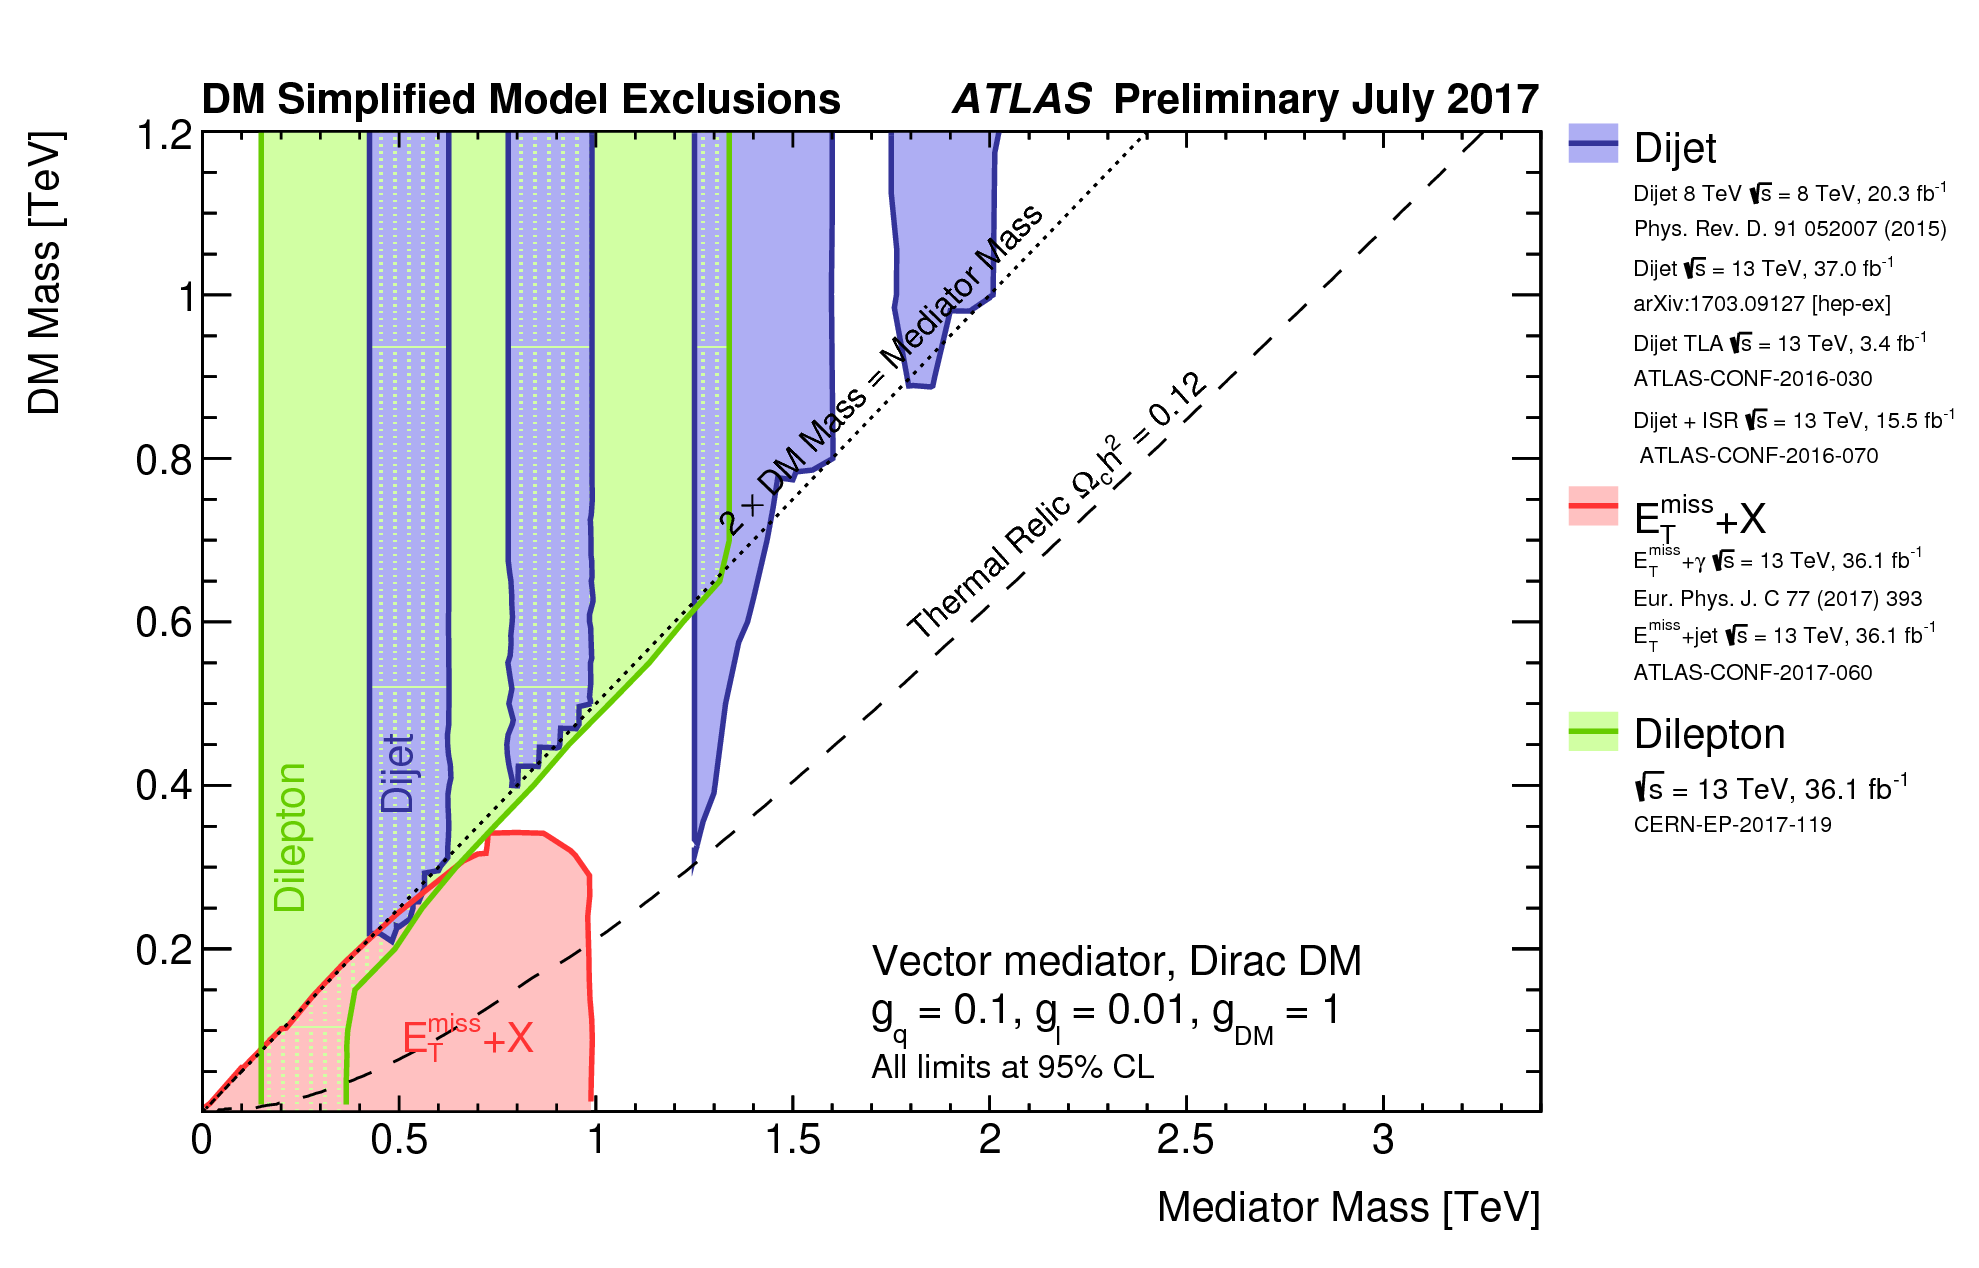
\includegraphics[width=\columnwidth]{figures/Conclusion/DMExclusions_Lepton.png}
%	\caption{Regions in a dark matter mass-mediator mass plane excluded at 95\% CL by a selection of ATLAS dark matter searches, for one possible interaction between the Standard Model and dark matter, the vector mediator as described in \cite{DMWorkingGroup}. The exclusions are computed for a dark matter coupling $g_{DM}$ = 1.0, a quark coupling $g_q$ = 0.1 universal to all flavors, and lepton coupling $g_l$ = 0.01, corresponding to the "V2" scenario in \cite{DMWorkingGroup}. With this choice of couplings, the $Z'$ decays to leptons are reduced with respect to the decays to quarks. The results use 13 TeV data except for \cite{DijetResonance8TeV_ATLAS}.  The lepton constraints use 13\,TeV data from 2016, reinterpreting the model independent limits in a way similar to what done for the dijet searches. The $E_T^{miss}$+X exclusion regions are obtained by rescaling, using acceptance and cross-section information from samples simulated at truth-level, the exclusion contours published in the corresponding papers. Dashed curves labeled "thermal relic" indicate combinations of dark matter and mediator mass that are consistent with a dark matter density of $\Omega_c = 0.12 h^2$  and a standard thermal history, as computed in MadDM (\cite{MadDM}, \cite{DMWorkingGroup}). To the left of the curve, annihilation processes described by the simplified model deplete $\Omega_c$ below 0.12 $h^2$. A dotted curve indicates the kinematic threshold where the mediator can decay on-shell into dark matter. The exclusion regions, relic density contours, and unitarity curve are not applicable to other choices of coupling values or model.}
%	\label{fig:DMExclusions_Lepton}
%\end{figure}
%
%Figure~\ref{fig:DMCouplings} shows a summary of the $Z'$ mediator limits in the plane of the resonance mass $m_{Z'}$ and coupling to quarks $g_q$ as of March 2018, reflecting the most recent results in the trigger-level analysis and boosted dijet + ISR searches.  These new results have greatly extended the lower mass reach and have bridged the gap between the masses covered by the high-mass search and the previous TLA result.  The Run-2 searches now cover a range from 100\,GeV to 3.5\,TeV, with exclusions ranging from 0.27 down to 0.04 in $g_q$.
%
%\begin{figure}[]
%	\centering
%	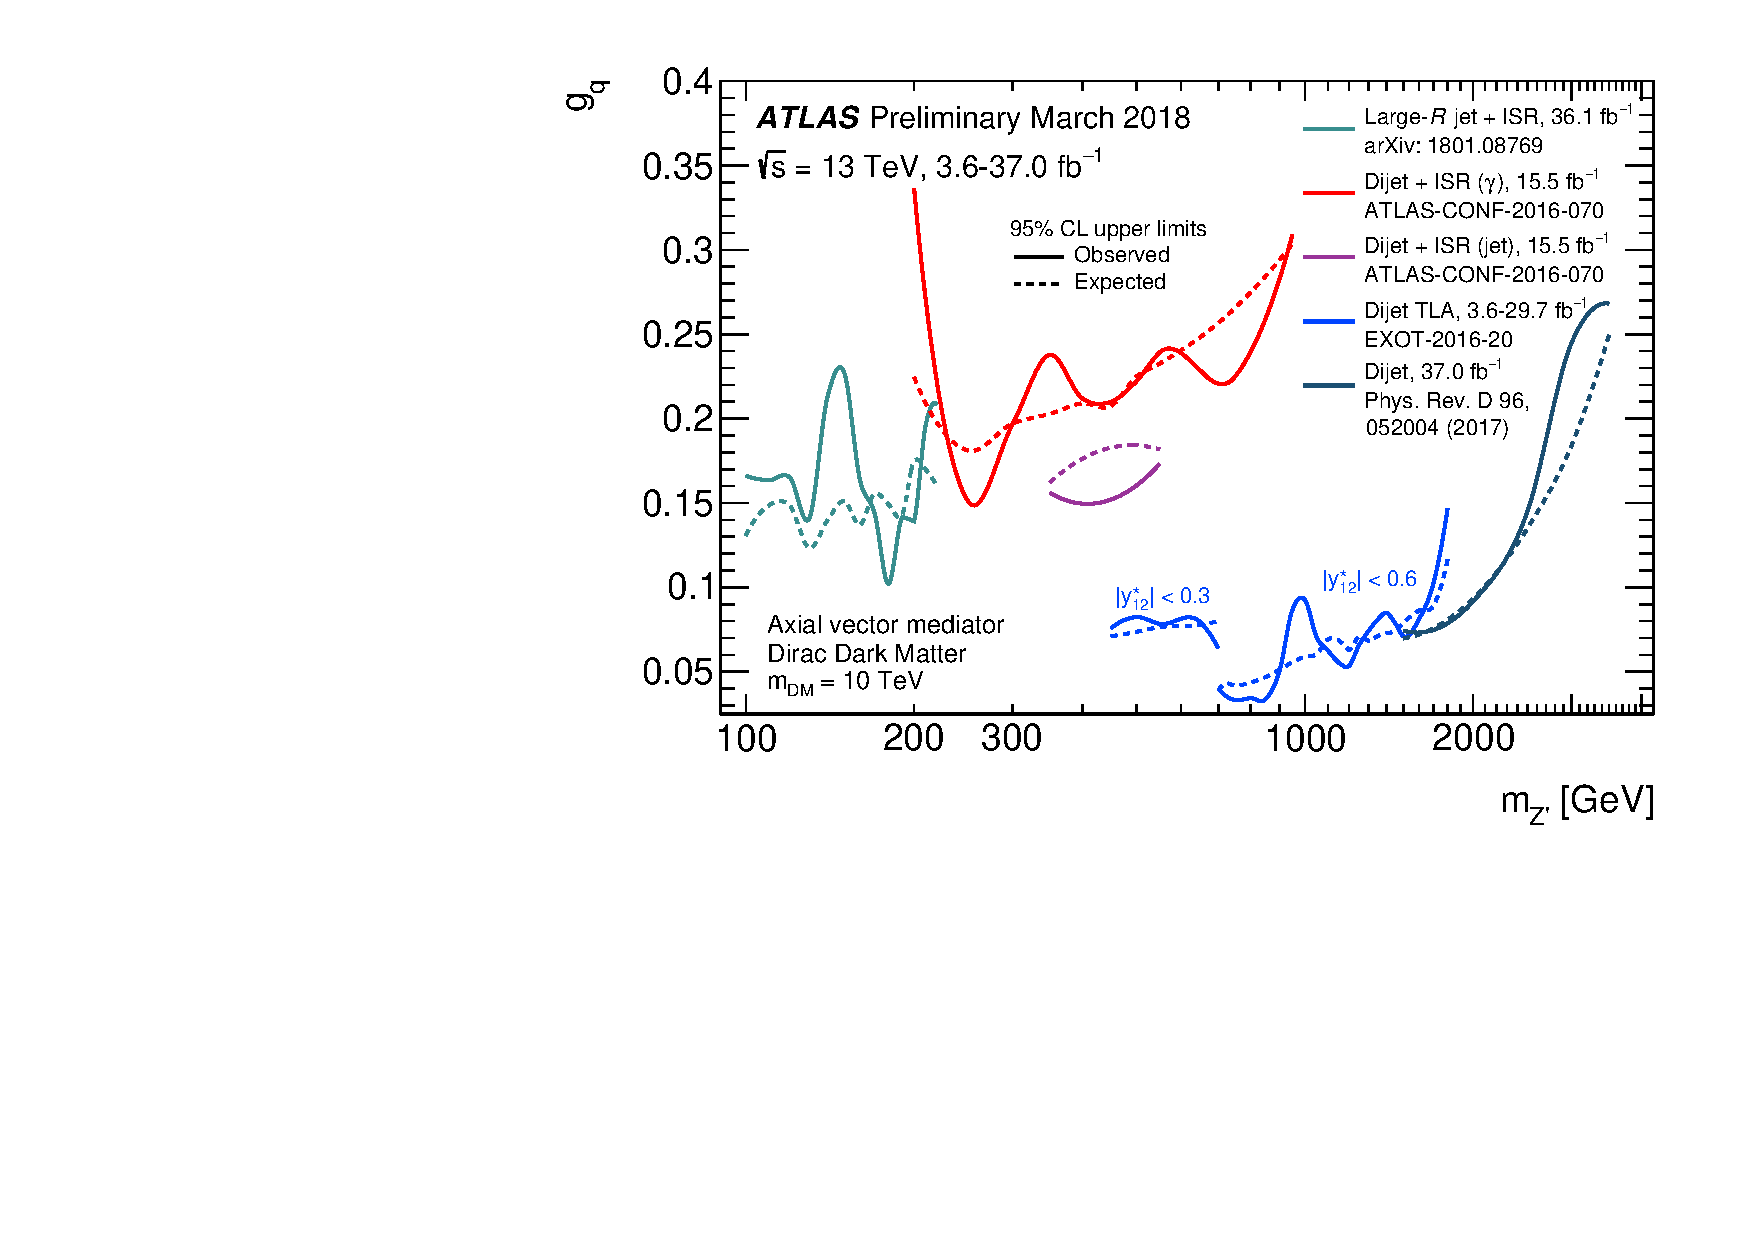
\includegraphics[width=\columnwidth]{figures/Conclusion/DMCouplings.pdf}
%	\caption{Summary plot of ATLAS bounds in the coupling-mediator mass plane from dijet searches using 2015 and 2016 data. The 95\% CL upper limits are on coupling $g_q$ as a function of the resonance mass $m_{Z'}$ for the leptophobic $Z'$ model described in \cite{DMForum}. The expected limits from each search are indicated by dotted curves. Coupling values above the solid curves are excluded, as long as the signals are narrow enough to be detected using these searches (10\% signal width/mass for dijet+ISR and TLA, 15\% for high-mass dijets, approximately corresponding to $g_q < 0.5$ and $g_q < 0.6$, respectively).}
%	\label{fig:DMCouplings}
%\end{figure}
%
%\section{Dijet Angular Search}
%
%In addition to the resonance bump hunt previously shown, ATLAS has also performed an angular shape analysis on dijet events, using the same event selection criteria but using events out to $|y^*|<1.7$, and cutting on the variable $y_B = |y_1+y_2|/2 < 1.1$.  Data is binned in both \mjj and in $\chi = e^{2|y^*|}$, and the $\chi$ distribution is compared to the shape expected from QCD as determined from simulated data.  Within each mass bin the shape is obtained from simulation and is scaled up to the amount of data seen.  The results of the angular search are shown in Figure~\ref{fig:AngularResult}.
%
%\begin{figure}[]
%	\centering
%	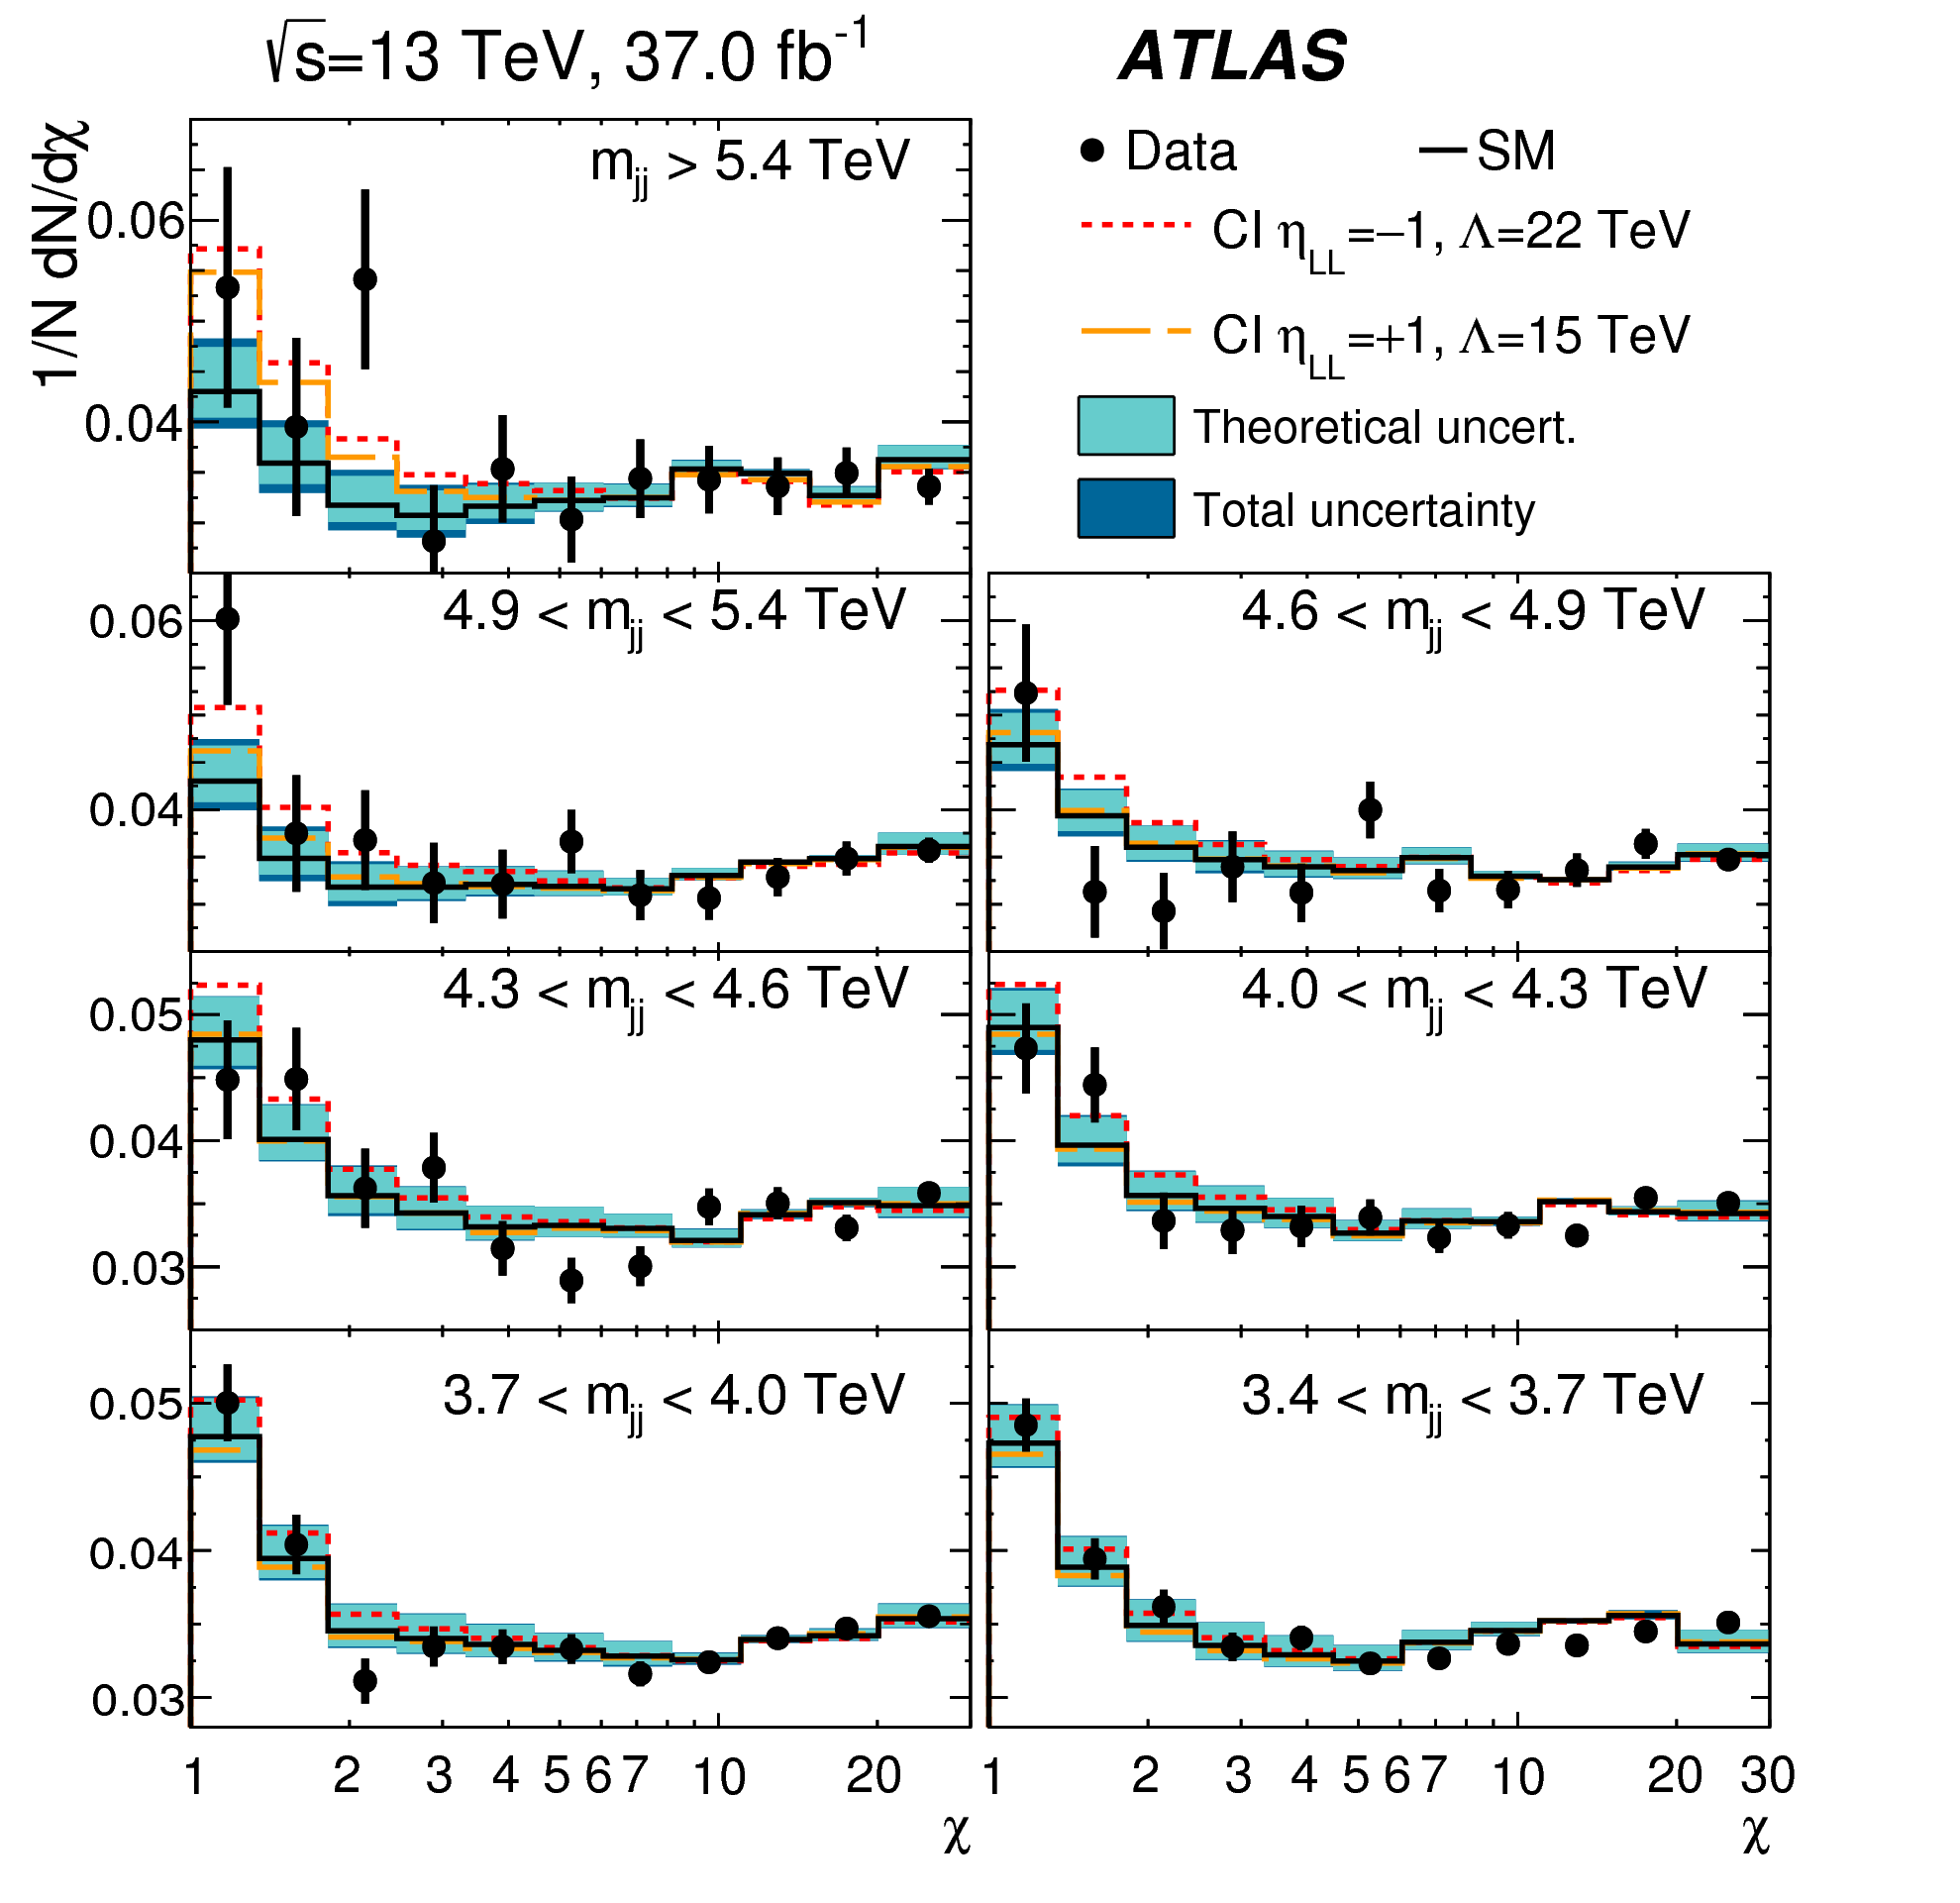
\includegraphics[width=\columnwidth]{figures/Conclusion/AngularResult.png}
%	\caption{Reconstructed distributions of the dijet angular variable $\chi$ in different regions of the dijet invariant mass \mjj. The data (points), Pythia predictions with NLO and electroweak corrections applied (solid lines), and examples of the contact interaction (CI) signals(dashed lines) are shown. The theoretical uncertainties and the total theoretical and experimental uncertainties in the predictions are displayed as shaded bands around the SM prediction. The SM background prediction and corresponding systematic uncertainty bands are extracted from the best-fit to the data. Data and predictions are normalized to unity in each \mjj~bin.}
%	\label{fig:AngularResult}
%\end{figure}
%
%While the ATLAS result is only interpreted in the context of limits on the scale of new quark contact interactions, they can also be extended to the same $Z'$ model, but can set limits for much higher values of $g_q$ as it is sensitive to much wider widths than the resonance search.  CMS has recently used their angular analysis~\cite{CMSAngular}~to set limits on the $Z'$ DM mediator model for very high mediator masses, the results of which are shown in Figure~\ref{fig:CMSZPrime}.  The results show a very large discrepancy from the expected limit for masses above 4.5~TeV; this may hint at a region of interest to be followed up on in the next resonance search, or may be due to a mis-modeling of the high invariant mass region by the simulated data which is used in this type of analysis.
%
%\begin{figure}[]
%	\centering
%	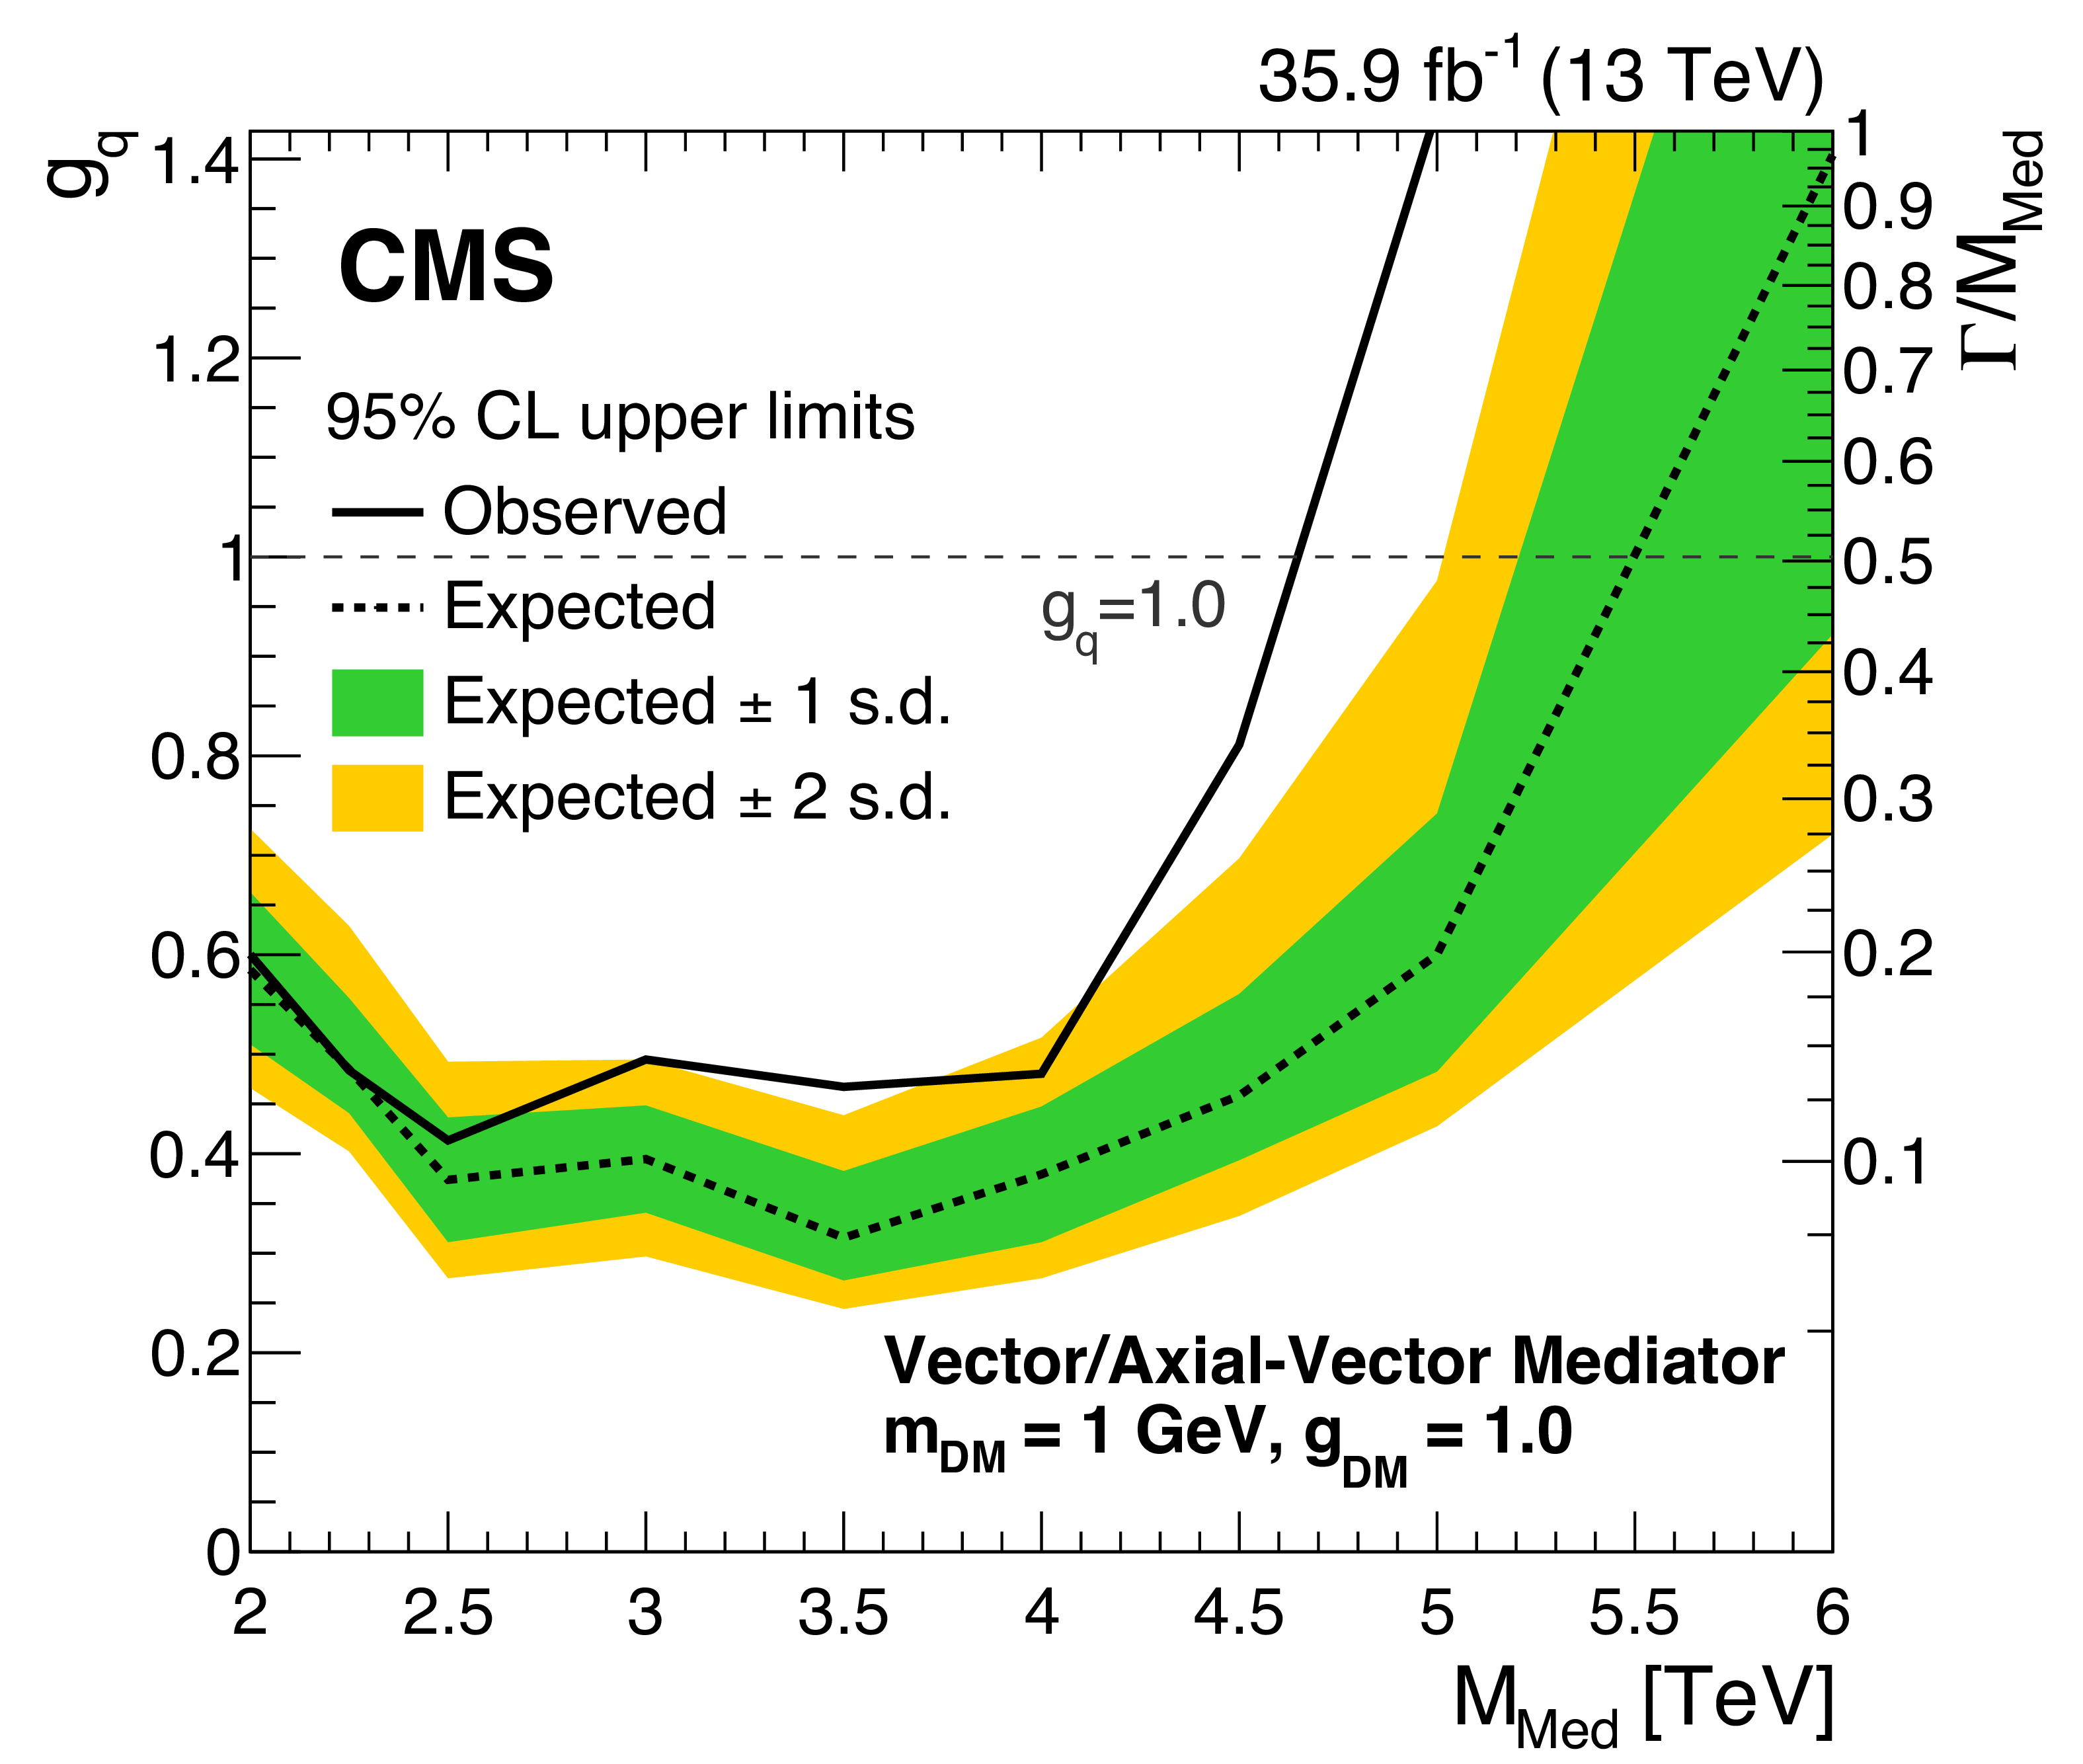
\includegraphics[width=\columnwidth]{figures/Conclusion/CMSZPrime.png}
%	\caption{Results from the CMS Collaboration showing the 95\% CL upper limits on the quark coupling $g_q$, as a function of mass, for an axial-vector or vector DM mediator with $g_{DM}$= 1.0 and $m_{DM}$= 1 GeV. The observed limits (solid), expected limits (dashed) and the variation in the expected limit at the 1 and 2 standard deviation levels (shaded bands) are shown. The corresponding limits on the width of the mediators are shown on the vertical axis on the right-hand side of the figure.\cite{CMSAngular}}
%	\label{fig:CMSZPrime}
%\end{figure}
%
%\section{Outlook}
%Looking forward, the next ATLAS publication will be on the complete Run-2 dataset, comprising some 100+\,\ifb of 13\,TeV data.  The LHC has already exceeded its design luminosity and expects to deliver even higher pileup in 2018, meaning that the ATLAS trigger menu must evolve to keep rates under control.  However, this evolution will have little impact on the dijet analysis, only requiring the loss of the lower one or two bins in the invariant mass spectrum.  The sensitivity of the dijet analysis is much more limited by the center-of-mass energy rather than by statistics, and as such minimal increases in limits are to be expected with the next paper result, with most benchmark models having their limits improve by 10\% or less. For comparison, the jump between the 2015 and 2015+2016 papers had 10$\times$ the integrated luminosity, but only improved limits between 9\% and 40\%.
%
%For the full HL-LHC dataset, comprising some 3000\,\ifb~at a center-of-mass energy of 14\,TeV, the expected limits on excited quarks and quantum black holes are estimated to be 8.0\,TeV and 10.1\,TeV, respectively. \cite{DijetOutlook}  Any increases beyond the design energy of the machine will lead to considerable improvements in these limits.
%
%\section{Conclusion}
%
%A search was performed analyzing dijet events in 37\,\ifb~of collision data with center-of-mass energy of 13\,TeV, taken with the ATLAS detector during the 2015 and 2016 runs.  The dijet invariant mass spectrum does not exhibit any excesses or deficits from the smoothly-falling background estimate which was obtained by a sliding window fit to the data.  The spectrum is also consistent with the spectrum derived from a simulation of QCD processes.  The most significant excess in the signal region has a p-value of 0.63, consistent with the background prediction.  The analysis sets limits on several benchmark signals, with an improvement of limits of 5-40\% in mass reach over the previous published limits by ATLAS in 2015 with 3.2\,\ifb~of data.
%
%
